% Options for packages loaded elsewhere
\PassOptionsToPackage{unicode}{hyperref}
\PassOptionsToPackage{hyphens}{url}
%
\documentclass[
  ignorenonframetext,
  serif,
  professionalfont,
  usenames,
  dvipsnames,
  aspectratio = 169]{beamer}
\usepackage{pgfpages}
\setbeamertemplate{caption}[numbered]
\setbeamertemplate{caption label separator}{: }
\setbeamercolor{caption name}{fg=normal text.fg}
\beamertemplatenavigationsymbolsempty
% Prevent slide breaks in the middle of a paragraph
\widowpenalties 1 10000
\raggedbottom
\setbeamertemplate{part page}{
  \centering
  \begin{beamercolorbox}[sep=16pt,center]{part title}
    \usebeamerfont{part title}\insertpart\par
  \end{beamercolorbox}
}
\setbeamertemplate{section page}{
  \centering
  \begin{beamercolorbox}[sep=12pt,center]{section title}
    \usebeamerfont{section title}\insertsection\par
  \end{beamercolorbox}
}
\setbeamertemplate{subsection page}{
  \centering
  \begin{beamercolorbox}[sep=8pt,center]{subsection title}
    \usebeamerfont{subsection title}\insertsubsection\par
  \end{beamercolorbox}
}
\AtBeginPart{
  \frame{\partpage}
}
\AtBeginSection{
  \ifbibliography
  \else
    \frame{\sectionpage}
  \fi
}
\AtBeginSubsection{
  \frame{\subsectionpage}
}
\usepackage{amsmath,amssymb}
\usepackage{iftex}
\ifPDFTeX
  \usepackage[T1]{fontenc}
  \usepackage[utf8]{inputenc}
  \usepackage{textcomp} % provide euro and other symbols
\else % if luatex or xetex
  \usepackage{unicode-math} % this also loads fontspec
  \defaultfontfeatures{Scale=MatchLowercase}
  \defaultfontfeatures[\rmfamily]{Ligatures=TeX,Scale=1}
\fi
\usepackage{lmodern}
\ifPDFTeX\else
  % xetex/luatex font selection
\fi
% Use upquote if available, for straight quotes in verbatim environments
\IfFileExists{upquote.sty}{\usepackage{upquote}}{}
\IfFileExists{microtype.sty}{% use microtype if available
  \usepackage[]{microtype}
  \UseMicrotypeSet[protrusion]{basicmath} % disable protrusion for tt fonts
}{}
\makeatletter
\@ifundefined{KOMAClassName}{% if non-KOMA class
  \IfFileExists{parskip.sty}{%
    \usepackage{parskip}
  }{% else
    \setlength{\parindent}{0pt}
    \setlength{\parskip}{6pt plus 2pt minus 1pt}}
}{% if KOMA class
  \KOMAoptions{parskip=half}}
\makeatother
\usepackage{xcolor}
\newif\ifbibliography
\usepackage{longtable,booktabs,array}
\usepackage{calc} % for calculating minipage widths
\usepackage{caption}
% Make caption package work with longtable
\makeatletter
\def\fnum@table{\tablename~\thetable}
\makeatother
\usepackage{graphicx}
\makeatletter
\newsavebox\pandoc@box
\newcommand*\pandocbounded[1]{% scales image to fit in text height/width
  \sbox\pandoc@box{#1}%
  \Gscale@div\@tempa{\textheight}{\dimexpr\ht\pandoc@box+\dp\pandoc@box\relax}%
  \Gscale@div\@tempb{\linewidth}{\wd\pandoc@box}%
  \ifdim\@tempb\p@<\@tempa\p@\let\@tempa\@tempb\fi% select the smaller of both
  \ifdim\@tempa\p@<\p@\scalebox{\@tempa}{\usebox\pandoc@box}%
  \else\usebox{\pandoc@box}%
  \fi%
}
% Set default figure placement to htbp
\def\fps@figure{htbp}
\makeatother
\setlength{\emergencystretch}{3em} % prevent overfull lines
\providecommand{\tightlist}{%
  \setlength{\itemsep}{0pt}\setlength{\parskip}{0pt}}
\setcounter{secnumdepth}{-\maxdimen} % remove section numbering
% Definição do esquema de cores:
% 1. UFPR - Azul com cinza.
% 2. DEST - Roxo com cinza.
% 3. LEG - Laranjado com cinza.
\def\mycolorscheme{1}

% Caminho para a imagem de fundo com aspecto 16x9.
% \def\pathtobg{config/ufpr-fachada-baixo-1.jpg}
% \def\pathtobg{config/ufpr-fundo.jpg}
% \def\pathtobg{config/ufpr-fundo.jpg}
\def\pathtobg{./config/ufpr-fundo-16x9.jpg}

% \providecommand{\tightlist}{%
%   \setlength{\itemsep}{0pt}\setlength{\parskip}{0pt}}
% ATTENTION: Redefine o comando acima que é definido pelo template.
% \renewcommand{\tightlist}{}
\renewcommand{\tightlist}{%
  \setlength{\itemsep}{0\baselineskip}
  \setlength{\parskip}{0.25\baselineskip}
}

% Logo na capa.
\titlegraphic{
  %\vspace{-1em}
  %
\includegraphics[height=1.2cm]{config/dest-texto-2.png}\hspace{1em}
  %\includegraphics[height=1.8cm]{config/dsbd-logo-2x2.png}\hspace{1em}
  
\includegraphics[height=1.8cm]{config/ufpr-transparent-600px.png}
}
%-----------------------------------------------------------------------

% Palladio.
% \usepackage[sc]{mathpazo}
% \linespread{1.05}         % Palladio needs more leading (space between lines)
% \usepackage[T1]{fontenc}

% Kurier.
% \usepackage[light, condensed, math]{kurier}
% \usepackage[T1]{fontenc}

% Iwona.
% \usepackage[math, light, condensed]{iwona}

% \usepackage{cmbright}
% \usepackage[charter]{mathdesign}
% \usepackage{palatino}

% Roboto (with Iwona for maths).
% \usepackage[math]{iwona}
% \usepackage[sfdefault, light, condensed]{roboto}

% Source Sans Pro (with Iwona for maths).
% \usepackage[math]{iwona}
% \usepackage[default, light]{sourcesanspro}

% Lato (with Iwona for maths).
% \usepackage[math]{iwona}
% \usepackage[default]{lato}

% Fira Sans (with Iwona for maths).
\usepackage[math, light]{iwona}
\usepackage[sfdefault,light]{FiraSans} %% option 'sfdefault' activates Fira Sans as the default text font
\usepackage[T1]{fontenc}
\renewcommand*\oldstylenums[1]{{\firaoldstyle #1}}

% Font for code. ----------------------------
% \usepackage[scaled=.75]{beramono}
\usepackage{inconsolata}

% ATTENTION: needs complile with xelatex: `$ xelatex file.tex`
% \usepackage{fontspec}
% \setmonofont{M+ 1m}
% \setmonofont{M+ 1mn}
% \setmonofont{M+ 2m}

%-----------------------------------------------------------------------

% \usepackage{lmodern}
\usepackage{amssymb, amsmath}
\usepackage[makeroom]{cancel}
% \usepackage{ifxetex, ifluatex}
\usepackage{fixltx2e} % provides \textsubscript
\usepackage[utf8]{inputenc}
\usepackage[shorthands=off,main=brazil]{babel}
\usepackage{graphicx}
\usepackage{xcolor}
\usepackage{setspace}
\usepackage{comment}
\usepackage{icomma}

%-----------------------------------------------------------------------
% Algumas configurações.

\setlength{\parindent}{0pt}
\setlength{\parskip}{6pt plus 2pt minus 1pt}
\setlength{\emergencystretch}{3em}  % prevent overfull lines
% \providecommand{\tightlist}{%
%   \setlength{\itemsep}{0pt}\setlength{\parskip}{0pt}}
\setcounter{secnumdepth}{0}

% Espaço vertical para o ambiente `quote`.
\let\oldquote\quote
\let\oldendquote\endquote
\renewenvironment{quote}{%
  \vspace{1em}\oldquote}{%
  \oldendquote\vspace{1em}}

%-----------------------------------------------------------------------
% Espaçamento entre items para itemize, enumerate e description.

% % itemize.
% \let\itemopen\itemize
% \let\itemclose\enditemize
% \renewenvironment{itemize}{%
%   \itemopen\addtolength{\itemsep}{0.25\baselineskip}}{\itemclose}
%
% % enumerate.
% \let\enumopen\enumerate
% \let\enumclose\endenumerate
% \renewenvironment{enumerate}{%
%   \enumopen\addtolength{\itemsep}{0.25\baselineskip}}{\enumclose}
%
% % description.
% \let\descopen\description
% \let\descclose\enddescription
% \renewenvironment{description}{%
%   \descopen\addtolength{\itemsep}{0.25\baselineskip}}{\descclose}

%-----------------------------------------------------------------------

% \usepackage[hang]{caption}
\usepackage{caption}
\captionsetup{font=footnotesize,
  labelfont={color=mycolor1, footnotesize},
  labelsep=period}

% \providecommand{\tightlist}{%
%   \setlength{\itemsep}{0pt}\setlength{\parskip}{0pt}}

%-----------------------------------------------------------------------

\usepackage{tikz}

% \def\pathtobg{/home/walmes/Projects/templates/COMMON/ufpr-fundo.jpg}
% \def\pathtobg{/home/walmes/Projects/templates/COMMON/ufpr-fundo-16x9.jpg}
% \def\pathtobg{/home/walmes/Projects/templates/COMMON/ufpr-fachada-dir-1.jpg}
% \def\pathtobg{/home/walmes/Projects/templates/COMMON/ufpr-fachada-esq-1.jpg}
% \def\pathtobg{/home/walmes/Projects/templates/COMMON/ufpr-perto-1.jpg}
% \def\pathtobg{/home/walmes/Projects/templates/COMMON/ufpr-fachada-baixo-1.jpg}

\ifx\pathtobg\undefined
\else
  \usebackgroundtemplate{
    \tikz[overlay, remember picture]
    \node[% opacity=0.3,
          at=(current page.south east),
          anchor=south east,
          inner sep=0pt] {
            \includegraphics[height=\paperheight, width=\paperwidth]{\pathtobg}};
  }
\fi

%-----------------------------------------------------------------------
% Definições de esquema de cores.

\ifx\mycolorscheme\undefined
  % UFPR.
  % http://www.color-hex.com/color-palette/2018
  \definecolor{mycolor1}{HTML}{015c93} % Título.
  \definecolor{mycolor2}{HTML}{363435} % Texto.
  \definecolor{mycolor3}{HTML}{015c93} % Estrutura.
  \definecolor{mycolor4}{HTML}{015c93} % Links.
  \definecolor{mycolor5}{HTML}{CECAC5} % Preenchimentos.
\else
  \if\mycolorscheme1
    % UFPR.
    \definecolor{mycolor1}{HTML}{015c93} % Título.
    \definecolor{mycolor2}{HTML}{363435} % Texto.
    \definecolor{mycolor3}{HTML}{015c93} % Estrutura.
    \definecolor{mycolor4}{HTML}{015c93} % Links.
    \definecolor{mycolor5}{HTML}{CECAC5} % Preenchimentos.
  \fi
  \if\mycolorscheme2
    % DEST.
    \definecolor{mycolor1}{HTML}{2a0e72} % Título.
    \definecolor{mycolor2}{HTML}{202E35} % Texto.
    \definecolor{mycolor3}{HTML}{2a0e72} % Estrutura.
    % \definecolor{mycolor3}{HTML}{8072a3} % Estrutura.
    \definecolor{mycolor4}{HTML}{2a0e72} % Links.
    % \definecolor{mycolor4}{HTML}{bfb9d1} % Links.
    % \definecolor{mycolor5}{HTML}{AEA79F} % Preenchimentos.
    \definecolor{mycolor5}{HTML}{CECAC5} % Preenchimentos.
  \fi
  \if\mycolorscheme3
    % LEG.
    \definecolor{mycolor2}{HTML}{363435} % Texto.
    % \definecolor{mycolor1}{HTML}{ff8000} % Título.
    % \definecolor{mycolor3}{HTML}{ff8000} % Estrutura.
    % \definecolor{mycolor4}{HTML}{ff8000} % Links.
    % \definecolor{mycolor1}{HTML}{E57300} % Título.
    % \definecolor{mycolor3}{HTML}{E57300} % Estrutura.
    % \definecolor{mycolor4}{HTML}{E57300} % Links.
    \definecolor{mycolor1}{HTML}{F67014} % Título.
    \definecolor{mycolor3}{HTML}{F67014} % Estrutura.
    \definecolor{mycolor4}{HTML}{F67014} % Links.
    % \definecolor{mycolor1}{HTML}{FE5C23} % Título.
    % \definecolor{mycolor3}{HTML}{FE5C23} % Estrutura.
    % \definecolor{mycolor4}{HTML}{FE5C23} % Links.
    \definecolor{mycolor5}{HTML}{222222} % Preenchimentos.
    \definecolor{mycolor5}{HTML}{383838} % Preenchimentos.
  \fi
\fi

\hypersetup{
  colorlinks=true,
  linkcolor=mycolor4,
  urlcolor=mycolor1,
  citecolor=mycolor1
}

%-----------------------------------------------------------------------
% ATTENTION: http://www.cpt.univ-mrs.fr/~masson/latex/Beamer-appearance-cheat-sheet.pdf

\usetheme{Boadilla}
\usecolortheme{default}

% \setbeamersize{text margin left=7mm, text margin right=7mm}
% \setbeamertemplate{frametitle}[default][left, leftskip=3mm]
% \addtobeamertemplate{frametitle}{\vspace{0.5em}}{}

\setbeamertemplate{caption}[numbered]
\setbeamertemplate{section in toc}[sections numbered]
\setbeamertemplate{subsection in toc}[subsections numbered]
\setbeamertemplate{sections/subsections in toc}[ball]{}
\setbeamertemplate{sections in toc}[ball]
\setbeamercolor{section number projected}{bg=mycolor1, fg=white}
\setbeamertemplate{blocks}[rounded]
\setbeamertemplate{navigation symbols}{}
\setbeamertemplate{frametitle continuation}{\gdef\beamer@frametitle{}}
% \setbeamertemplate{frametitle}[default][center]
% \setbeamertemplate{footline}[frame number]

\setbeamertemplate{enumerate items}[default]
\setbeamertemplate{itemize items}{\scriptsize\raise1.25pt\hbox{\donotcoloroutermaths$\blacktriangleright$}}

% Blocos.
% \addtobeamertemplate{block begin}{\vskip -\bigskipamount}{}
% \addtobeamertemplate{block end}{}{\vskip -\bigskipamount}
\addtobeamertemplate{block begin}{\vspace{0.5em}}{}
\addtobeamertemplate{block end}{}{\vspace{0.5em}}


% Rodapé.
\setbeamercolor{title in head/foot}{parent=subsection in head/foot}
\setbeamercolor{author in head/foot}{bg=mycolor4, fg=white}
\setbeamercolor{date in head/foot}{parent=subsection in head/foot, fg=mycolor3}

% Cabeçalho.
\setbeamercolor{section in head/foot}{bg=mycolor2, fg=mycolor4}
\setbeamercolor{subsection in head/foot}{bg=mycolor2, fg=white}

\setbeamercolor{title}{fg=mycolor1}       % Título dos slides.
\setbeamercolor{titlelike}{fg=title}
\setbeamercolor{subtitle}{fg=mycolor2}    % Subtítulo.
\setbeamercolor{institute in head/foot}{parent=palette primary} % Instituição.
\setbeamercolor{frametitle}{fg=mycolor1}  % De quadro.
\setbeamercolor{structure}{fg=mycolor3}   % Listas e rodapé.
\setbeamercolor{item projected}{bg=mycolor2}
\setbeamercolor{block title}{bg=mycolor5, fg=mycolor2}
\setbeamercolor{normal text}{fg=mycolor2} % Texto.
\setbeamercolor{caption name}{fg=normal text.fg}
% \setbeamercolor{footlinecolor}{fg=mycolor2, bg=mycolor5}
% \setbeamercolor{section in head/foot}{fg=mycolor2, bg=mycolor5}
\setbeamercolor{author in head/foot}{fg=white, bg=mycolor1}
\setbeamercolor{section in foot}{fg=mycolor4, bg=mycolor5}
\setbeamercolor{date in foot}{fg=mycolor4, bg=mycolor5}
\setbeamercolor{block title}{fg=white, bg=mycolor1}
\setbeamercolor{block body}{fg=black, bg=white!80!gray}
\setbeamercolor{block body}{fg=black, bg=white!80!gray}

% To remove empty brackets of \institution.
\makeatletter
\setbeamertemplate{footline}{
  \leavevmode%
  \hbox{%
    \begin{beamercolorbox}[
      wd=0.3\paperwidth, ht=2.25ex, dp=1ex, right]{author in head/foot}%
      \usebeamerfont{author in head/foot}\insertshortauthor{}\hspace*{1ex}
    \end{beamercolorbox}%
    \begin{beamercolorbox}[
      wd=0.6\paperwidth, ht=2.25ex, dp=1ex, left]{section in foot}%
      \usebeamerfont{title in head/foot}\hspace*{1ex}\insertshorttitle{}
      % \usebeamerfont{title in head/foot}\hspace*{1ex}\insertframetitle{}
    \end{beamercolorbox}%
    \begin{beamercolorbox}[
      wd=0.1\paperwidth, ht=2.25ex, dp=1ex, right]{date in foot}%
      \insertframenumber{}\hspace*{2ex}
    \end{beamercolorbox}
  }%
  \vskip0pt%
}
\makeatother

%-----------------------------------------------------------------------

% \usepackage{hyphenat}
\usepackage{changepage}

% Slide para o título das seções.
\AtBeginSection[]{
  \begin{frame}
    % \vfill
    \vspace{4cm}
    % \centering
    % \begin{beamercolorbox}[sep = 8pt, center, shadow = true, rounded = true]{title}
    \begin{beamercolorbox}{title}
      \begin{columns}
        \column{0.7\linewidth}
        {\LARGE\textbf \insertsectionhead}
      \end{columns}
    \end{beamercolorbox}
    \vfill
  \end{frame}
}

%-----------------------------------------------------------------------
%---- preamble-chunk.tex -----------------------------------------------

% Knitr.

% ATTENTION: this needs `\usepackage{xcolor}'.
\definecolor{color_line}{HTML}{333333}
\definecolor{color_back}{HTML}{DDDDDD}
% \definecolor{color_back}{HTML}{FF0000}

% ATTENTION: usa o fancyvrb.
% https://ctan.math.illinois.edu/macros/latex/contrib/fancyvrb/doc/fancyvrb-doc.pdf
% R input.
\usepackage{tcolorbox}
\ifcsmacro{Highlighting}{
  % Statment if it exists. ------------------
  \DefineVerbatimEnvironment{Highlighting}{Verbatim}{
    % frame=lines,     % Linha superior e inferior.
    % framerule=0.5pt, % Espessura da linha.
    framesep=2ex,    % Distância da linha para o texto.
    % rulecolor=\color{color_line},
    % numbers=right,
    fontsize=\footnotesize, % Tamanho da fonte.
    baselinestretch=0.8,    % Espaçamento entre linhas.
    commandchars=\\\{\}}
  % Margens do ambiente `Shaded'.
  % \fvset{listparameters={\setlength{\topsep}{-1em}}}
  % \renewenvironment{Shaded}{\vspace{-1ex}}{\vspace{-2ex}}
  \renewenvironment{Shaded}{
    \vspace{2pt}
    \begin{tcolorbox}[
      boxrule=0pt,      % Espessura do contorno.
      colframe=gray!10, % Cor do contorno.
      colback=gray!10,  % Cor de fundo da caixa.
      arc=1em,          % Raio para contornos arredondados.
      sharp corners,
      boxsep=0.5em,     % Margem interna.
      left=3pt, right=3pt, top=3pt, bottom=3pt, % Margens internas.
      grow to left by=0mm,
      grow to right by=6pt,
      ]
    }{
    \end{tcolorbox}
    \vspace{-3pt}
    }
  }{
  % Statment if it not exists. --------------
}

% R output e todo `verbatim'.
\makeatletter
\def\verbatim@font{\linespread{0.8}\ttfamily\footnotesize}
%\makeatother

% Cor de fundo e margens do `verbatim'.
\let\oldv\verbatim
\let\oldendv\endverbatim

\def\verbatim{%
  \par\setbox0\vbox\bgroup % Abre grupo.
  %\vspace{-5px}            % Reduz margem superior.
  \oldv                    % Chama abertura do verbatim.
}
\def\endverbatim{%
  \oldendv                 % Chama encerramento do verbatim.
  %\vspace{0cm}           % Controla margem inferior.
  \egroup%\fboxsep5px      % Fecha grupo.
  \noindent{{\usebox0}}\par
}

%-----------------------------------------------------------------------
%---- preamble-commands.tex --------------------------------------------

% Para fazer texto em duas colunas.
\newcommand{\mytwocolumns}[4]{
  % #1: Line width fraction for the left column , e.g. 0.5.
  % #2: Line width fraction for the right column.
  % #3: Content for the left column.
  % #4: Content for the right column.
  \begin{columns}[c]
    \begin{column}{#1\linewidth} %----------- left.
      #3
    \end{column} %--------------------------- left.
    \begin{column}{#2\linewidth} %----------- right.
      #4
    \end{column} %--------------------------- right.
  \end{columns}
}

%-----------------------------------------------------------------------
% Para fazer duas colunas no Rmd.

% Center vertical align.
\def\beginAHalfColumn{\begin{minipage}{0.49\textwidth}}%
\def\beginAlmostHalfColumn{\begin{minipage}{0.45\textwidth}}%
\def\beginAQuarterColumn{\begin{minipage}{0.23\textwidth}}%
\def\beginThreeQuartersColumn{\begin{minipage}{0.72\textwidth}}%
\def\beginAThirdColumn{\begin{minipage}{0.31\textwidth}}%
\def\beginTwoThirdsColumn{\begin{minipage}{0.64\textwidth}}%
\def\endColumns{\end{minipage}}%

% Top vertical align.
\def\beginAHalfColumnT{\begin{minipage}[t]{0.49\textwidth}}%
\def\beginAlmostHalfColumnT{\begin{minipage}[t]{0.45\textwidth}}%
\def\beginAQuarterColumnT{\begin{minipage}[t]{0.23\textwidth}}%
\def\beginThreeQuartersColumnT{\begin{minipage}[t]{0.72\textwidth}}%
\def\beginAThirdColumnT{\begin{minipage}[t]{0.31\textwidth}}%
\def\beginTwoThirdsColumnT{\begin{minipage}[t]{0.64\textwidth}}%

%---------------------------------------------------------------------
% Ambientes para frases como e sem imagem.

\newcommand{\myquote}[3]{
  % #1: caminho para a imagem.
  % #2: a frase/quotation.
  % #3: o autor.
  \begin{center}
    \begin{minipage}[c]{0.19\linewidth}
      \begin{center}
        \includegraphics[height=2.5cm]{#1}
      \end{center}
    \end{minipage}
    \begin{minipage}[c]{0.7\linewidth}
      \begin{flushright}
        \textit{#2}
        \vspace{1ex}

        -- #3
      \end{flushright}
    \end{minipage}
  \end{center}
}

\newcommand{\myphrase}[2]{
  % #1: a frase/quotation.
  % #2: o autor.
  \begin{center}
    \begin{minipage}[c]{0.19\linewidth}
    \end{minipage}
    \begin{minipage}[c]{0.7\linewidth}
      \begin{flushright}
        \textit{#1}
        \vspace{1ex}

        -- #2
      \end{flushright}
    \end{minipage}
  \end{center}
}

%-----------------------------------------------------------------------
% Comandos para texto em destaque.

% \newcommand{\hi}[1]{%
%   \textcolor{ubuntu_orange}{#1}\xspace
% }

\usepackage{xspace}

% URLs com letra miuda.
\newcommand{\myurl}[1]{%
  {\tiny \url{#1}}\xspace
}

% Botões.
\newcommand{\btn}[1]{%
  \beamergotobutton{#1}\xspace
}

% Texto grande centralizado.
\newcommand{\centertitle}[1]{%
  \begin{center}
    {\LARGE \bfseries \hi{#1}}
  \end{center}
}

%-----------------------------------------------------------------------
\usepackage{bookmark}
\IfFileExists{xurl.sty}{\usepackage{xurl}}{} % add URL line breaks if available
\urlstyle{same}
\hypersetup{
  pdfauthor={Prof.~Me. Lineu Alberto Cavazani de Freitas },
  hidelinks,
  pdfcreator={LaTeX via pandoc}}

\title{\hfill\break
\textbf{Fundamentos de Análise Exploratória de Dados}\\
Conceitos e Aplicações}
\subtitle{\hfill\break
Encontro 2\\
Resumos numéricos e análises bivariadas.}
\author{Prof.~Me. Lineu Alberto Cavazani de Freitas \vspace{-0.5cm}}
\date{}

\begin{document}
\frame{\titlepage}

\begin{frame}{Análise exploratória}
\phantomsection\label{anuxe1lise-exploratuxf3ria}
\begin{itemize}
\item
  Parte primordial de qualquer análise estatística é chamada
  \textbf{análise descritiva} ou \textbf{exploratória}.
\item
  Consiste basicamente de \textbf{tabelas}, \textbf{resumos numéricos} e
  \textbf{análises gráficas} das variáveis disponíveis em um conjunto de
  dados.
\item
  Trata-se de uma etapa de extrema importância e deve preceder qualquer
  análise mais sofisticada.
\item
  As técnicas de análise exploratória visam \textbf{resumir} e
  \textbf{apresentar} as informações de um conjunto de dados brutos.
\end{itemize}
\end{frame}

\begin{frame}{Análise exploratória}
\phantomsection\label{anuxe1lise-exploratuxf3ria-1}
\beginAHalfColumn

\begin{itemize}
\tightlist
\item
  A análise exploratória de dados é uma área relativamente nova.
\end{itemize}

\vspace{0.3cm}

\begin{itemize}
\tightlist
\item
  Nasceu do clássico livro \textbf{Exploratory Data Analysis} de
  \textbf{John Tukey} em 1977.
\end{itemize}

\vspace{0.3cm}

\begin{itemize}
\tightlist
\item
  Algo curioso é que Tukey tinha uma relação próxima com a Ciência da
  Computação e definiu os termos \textbf{bit} e \textbf{software}.
\end{itemize}

\endColumns
\beginAHalfColumn

\begin{figure}

{\centering 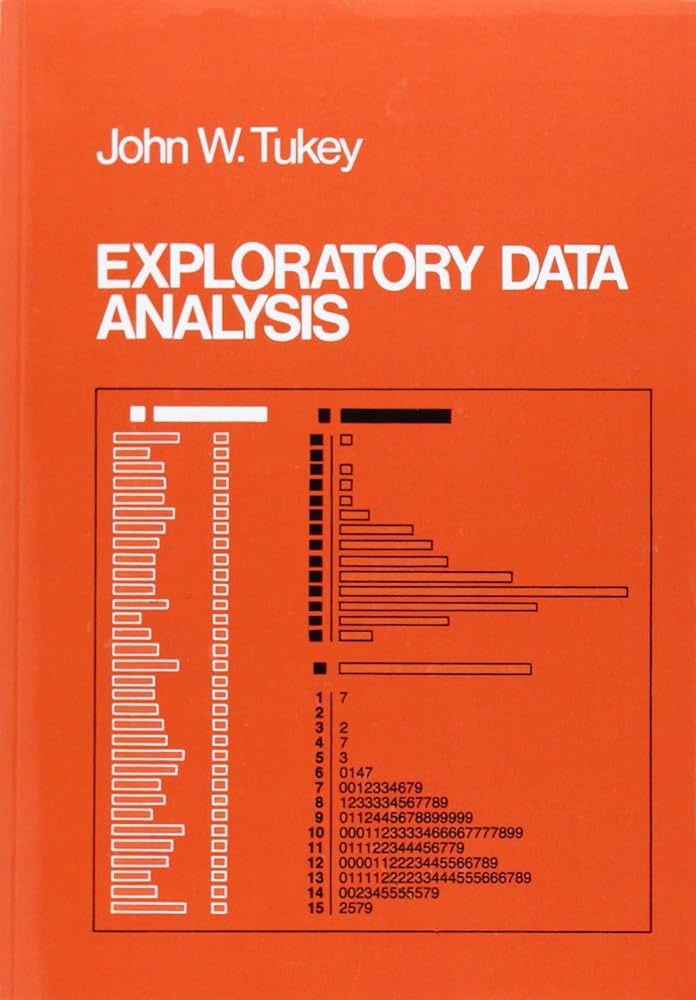
\includegraphics[width=0.62\linewidth]{./img/eda-tukey} 

}

\caption{Capa do livro Exploratory Data Analysis de John Tukey.}\label{fig:unnamed-chunk-2}
\end{figure}

\endColumns
\end{frame}

\begin{frame}{Análise exploratória}
\phantomsection\label{anuxe1lise-exploratuxf3ria-2}
\begin{itemize}
\item
  Como quase tudo em análise de dados, o \textbf{avanço computacional}
  permitiu com que a análise exploratória evoluísse substancialmente.
\item
  Por exemplo: historicamente o processo de criação de um gráfico era
  reservado a pessoas qualificadas pois a produção de uma visualização
  era difícil.
\item
  Hoje qualquer pessoa pode inserir dados em um aplicativo e gerar um
  gráfico.
\item
  Este tipo de facilidade é importante para disseminação e
  democratização dos métodos, porém abre margem para certas práticas
  inadequadas.
\end{itemize}
\end{frame}

\begin{frame}{Análise exploratória}
\phantomsection\label{anuxe1lise-exploratuxf3ria-3}
\beginAHalfColumn

\begin{itemize}
\tightlist
\item
  Tentar compreender um conjunto de dados sem algum método que permita
  resumir as informações é inviável.
\end{itemize}

\vspace{0.3cm}

\begin{itemize}
\tightlist
\item
  A análise exploratória é a primeira forma de tentarmos entender o que
  acontece nos nossos dados.
\end{itemize}

\vspace{0.3cm}

\begin{itemize}
\tightlist
\item
  Uma das tarefas é a etapa de consistência dos dados, isto é, verificar
  se os dados coletados são condizentes com a realidade.
\end{itemize}

\endColumns
\beginAHalfColumn

\begin{figure}

{\centering 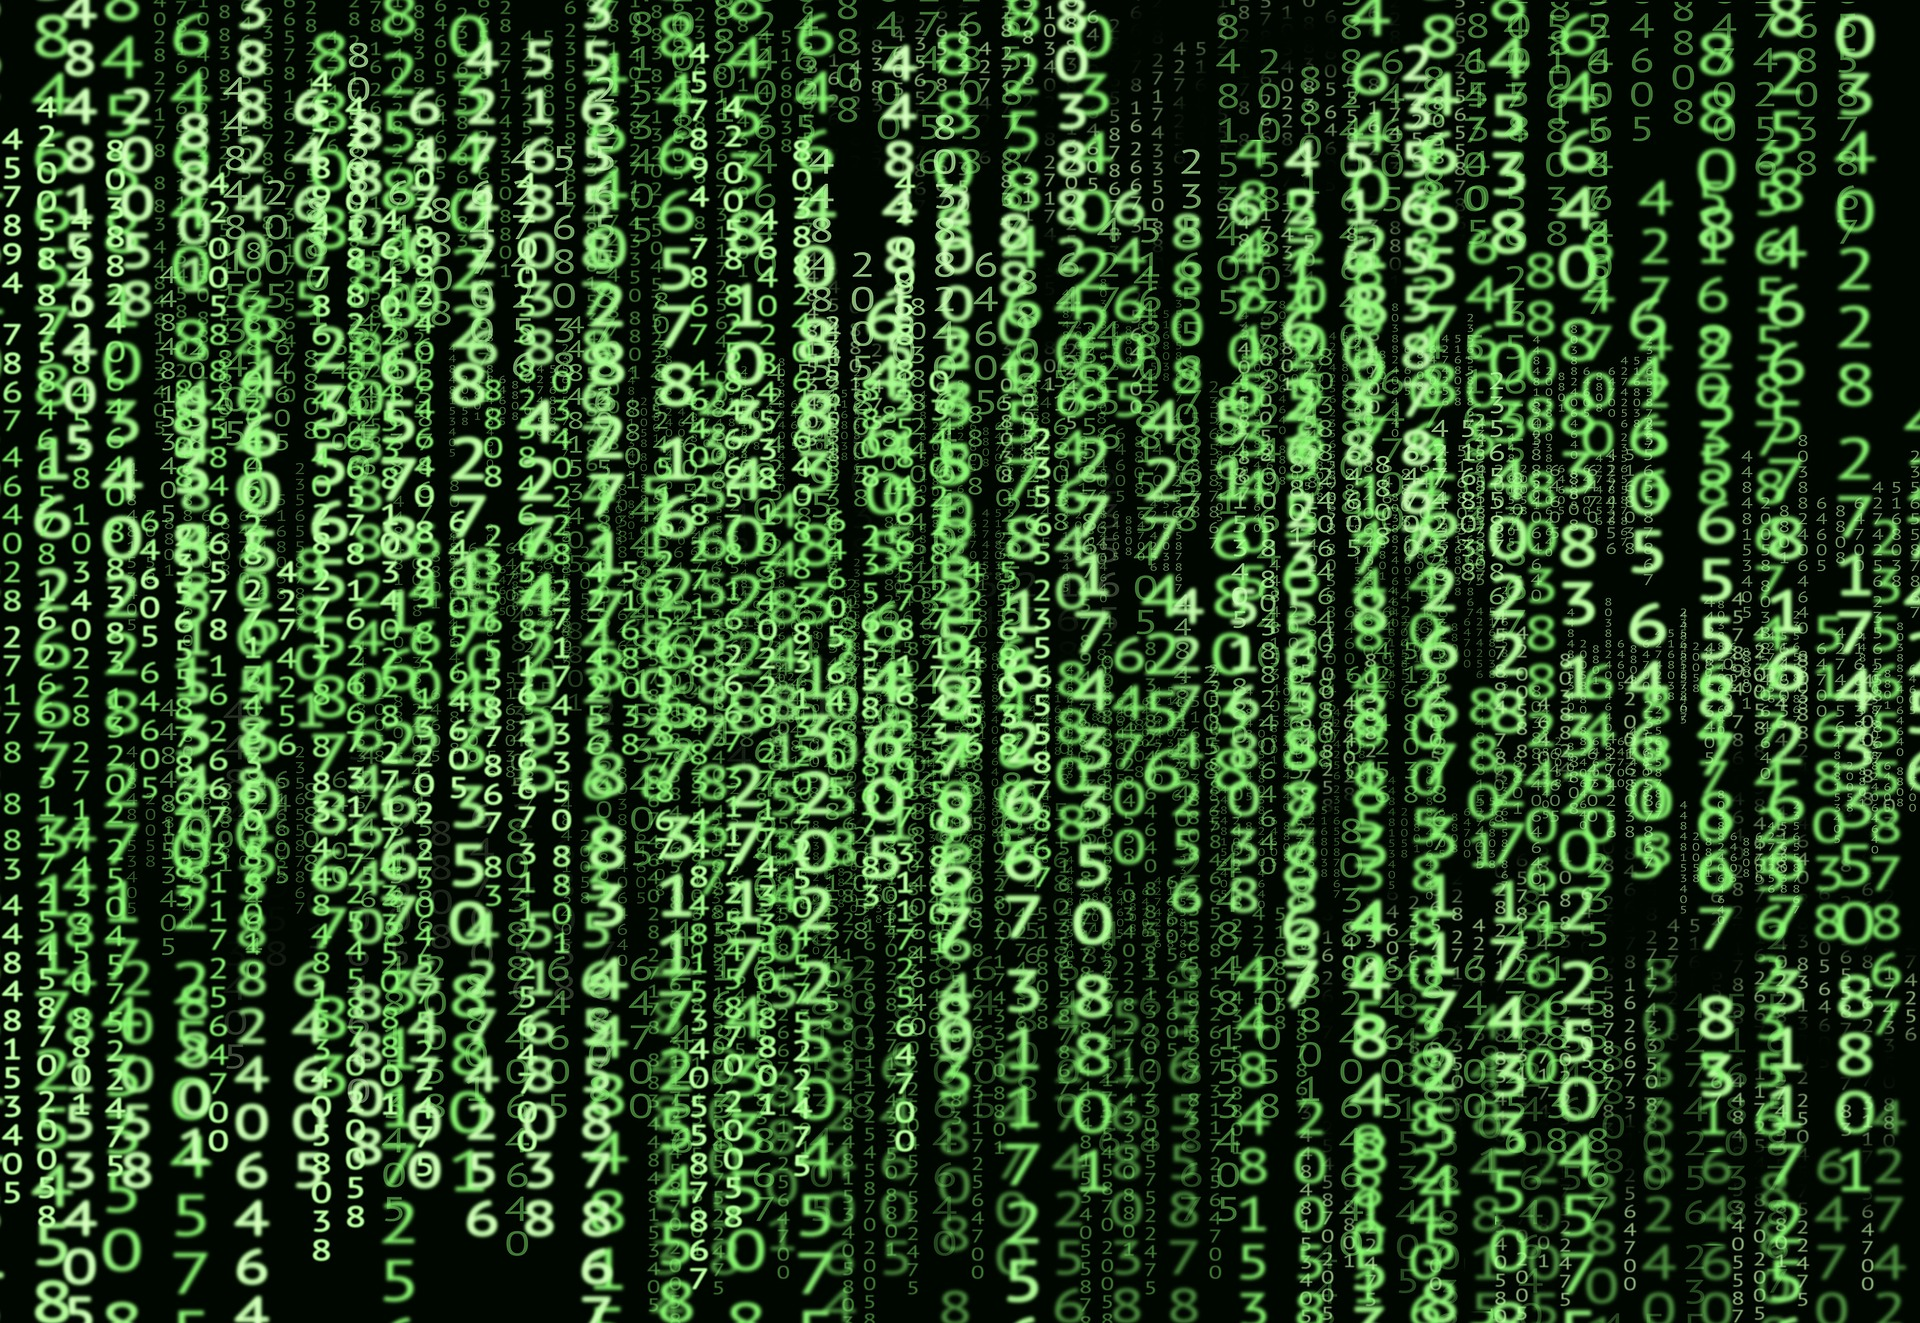
\includegraphics[width=0.9\linewidth]{./img/dados} 

}

\caption{Extraído de \href{https://cdn.pixabay.com/photo/2018/01/26/18/21/matrix-3109378_1280.jpg}{pixabay.com.}}\label{fig:unnamed-chunk-3}
\end{figure}

\endColumns
\end{frame}

\begin{frame}{Análise exploratória}
\phantomsection\label{anuxe1lise-exploratuxf3ria-4}
\beginAHalfColumn

\begin{itemize}
\tightlist
\item
  O conjunto de técnicas aplicáveis está diretamente associado ao
  \textbf{tipo das variáveis de interesse} (quantitativas x
  qualitativas) e suas ramificações.
\end{itemize}

\vspace{0.3cm}

\begin{itemize}
\tightlist
\item
  Podemos conduzir análises focadas nas variáveis uma a uma
  (\textbf{análises univariadas}).
\end{itemize}

\vspace{0.3cm}

\begin{itemize}
\tightlist
\item
  Também podemos conduzir análises focadas em avaliar a relação entre as
  variáveis (\textbf{análises multivariadas}).
\end{itemize}

\endColumns
\beginAHalfColumn

\begin{figure}

{\centering 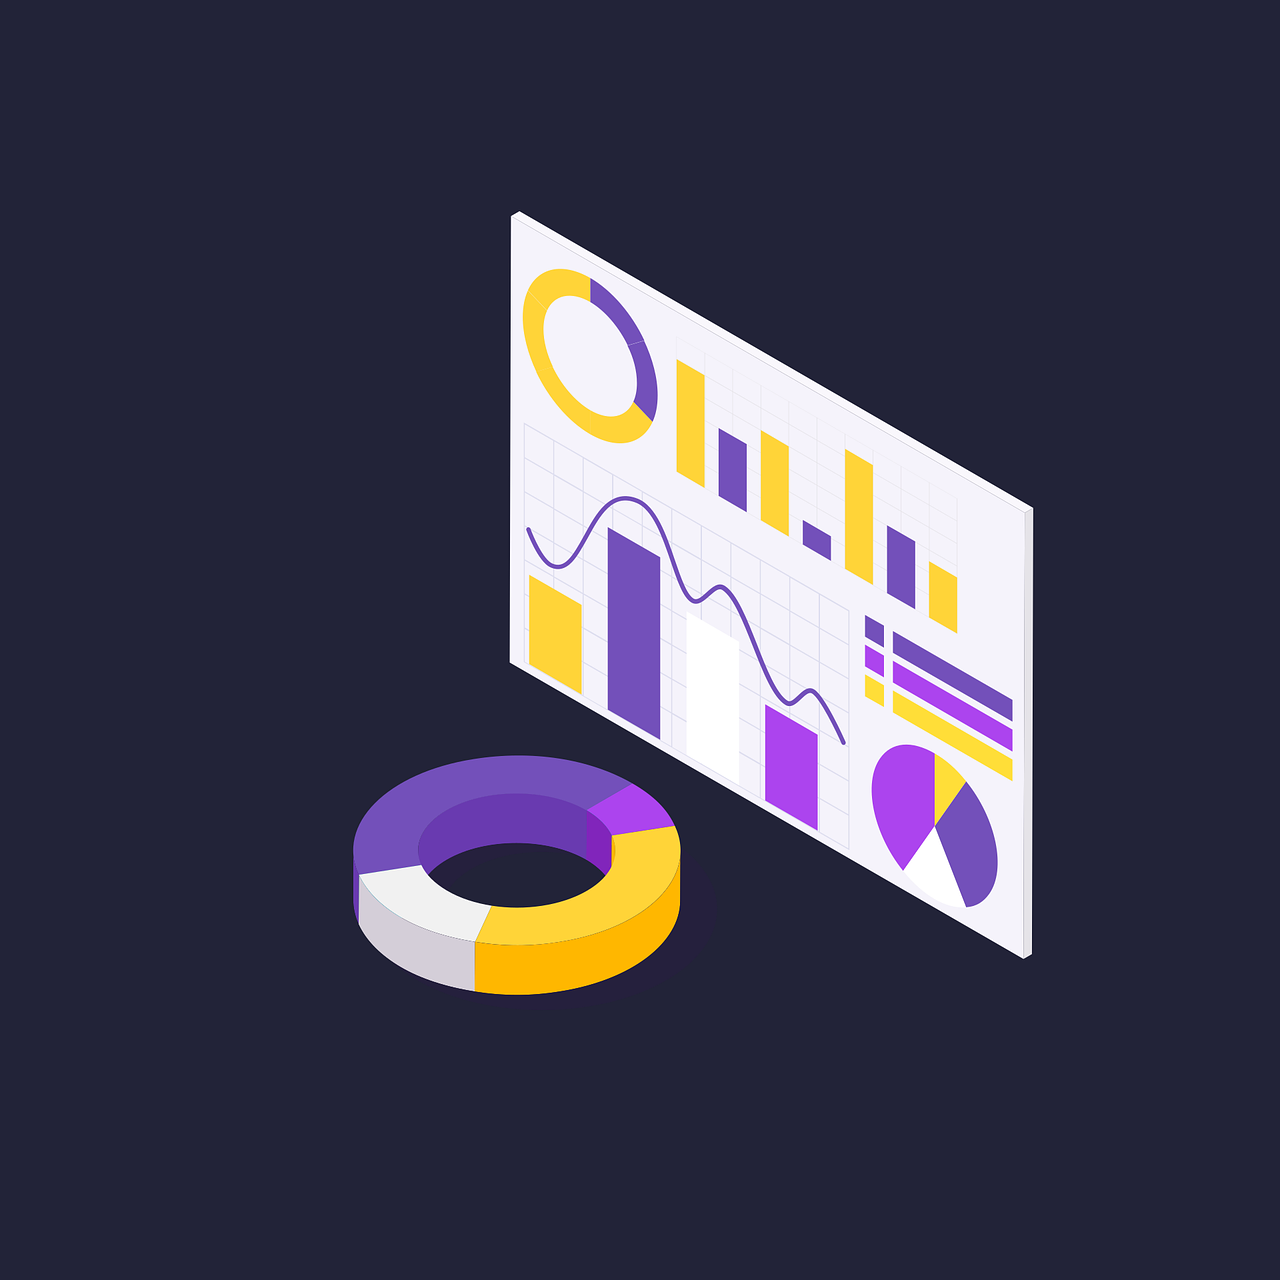
\includegraphics[width=0.8\linewidth]{./img/exploratoria} 

}

\caption{Extraído de \href{https://cdn.pixabay.com/photo/2020/08/03/10/00/graph-5459708_1280.png}{pixabay.com.}}\label{fig:unnamed-chunk-4}
\end{figure}

\endColumns
\end{frame}

\begin{frame}{Análise exploratória}
\phantomsection\label{anuxe1lise-exploratuxf3ria-5}
Podemos fazer uso diversas técnicas, tais como

\beginAHalfColumn

\begin{itemize}
\tightlist
\item
  Tabelas de frequência absolutas.
\item
  Tabelas de frequência relativas.
\item
  Tabelas de frequência acumuladas.
\item
  Tabelas para múltiplas variáveis.
\item
  Gráficos.
\end{itemize}

\endColumns
\beginAHalfColumn

\begin{itemize}
\tightlist
\item
  Medidas de posição central.
\item
  Medidas de posição relativa.
\item
  Medidas de forma.
\item
  Medidas de dispersão.
\item
  Medidas de associação.
\end{itemize}

\endColumns
\end{frame}

\section{Resumos numéricos}\label{resumos-numuxe9ricos}

\begin{frame}{Resumos numéricos}
\phantomsection\label{resumos-numuxe9ricos-1}
\begin{itemize}
\item
  Uma forma de resumir a informação contida em um conjunto de dados é
  por meio dos \textbf{resumos numéricos}.
\item
  Resumos numéricos são basicamente
  \textbf{números que resumem números}.
\item
  Os dois principais grupos são as medidas de \textbf{posição} (central
  e relativa) e \textbf{dispersão}.
\item
  Existem outros conjuntos de medidas, como as medidas de \textbf{forma}
  e também as de \textbf{relação/associação}.
\end{itemize}
\end{frame}

\section{Medidas de posição
central}\label{medidas-de-posiuxe7uxe3o-central}

\begin{frame}{Medidas de posição central}
\phantomsection\label{medidas-de-posiuxe7uxe3o-central-1}
\begin{itemize}
\item
  Um passo fundamental na exploração dos dados é definir um
  \textbf{valor típico} (uma estimativa onde a maior parte dos dados
  está localizada).
\item
  Considerando um conjunto de valores qualquer, como definir um valor
  central? A resposta é: depende do critério.
\end{itemize}

\vspace{0.7cm}

\beginAHalfColumn

\begin{itemize}
\tightlist
\item
  As medidas de posição central buscam expressar o \textbf{centro} de
  uma variável por meio de ideias como:

  \begin{itemize}
  \tightlist
  \item
    Centro de massa.
  \item
    Valor que divide a amostra em partes iguais.
  \item
    Valores de maior frequência ou densidade.
  \end{itemize}
\end{itemize}

\endColumns
\beginAHalfColumn

\begin{itemize}
\tightlist
\item
  Algumas possiblidades são

  \begin{itemize}
  \tightlist
  \item
    Média.
  \item
    Mediana.
  \item
    Moda.
  \item
    Média geométrica.
  \item
    Média harmônica.
  \item
    Média aparada.
  \end{itemize}
\end{itemize}

\endColumns
\end{frame}

\begin{frame}{Média aritmética}
\phantomsection\label{muxe9dia-aritmuxe9tica}
\begin{itemize}
\tightlist
\item
  Soma de todos os valores dividida pela quantidade de elementos.
\item
  Interpretação física de centro de gravidade.
\item
  Medida influenciada por valores extremos.
\end{itemize}

\textbf{Expressão}

Sejam \(y_1, y_2,...,y_n\) os \(n\) valores de uma variável \(Y\), a
média é dada por:

\[
      \overline{y} = \dfrac{\sum_{i = 1}^{n} y_i}{n} = \frac{y_1 + y_2 + \cdots + y_n}{n}.
\]
\end{frame}

\begin{frame}{Média aritmética}
\phantomsection\label{muxe9dia-aritmuxe9tica-1}
\textbf{Exemplo}

\begin{itemize}
\item
  Considere que uma turma possui 10 alunos.
\item
  Estes alunos realizaram uma avaliação.
\item
  Considere que as notas obtidas foram:
\end{itemize}

\[60;\ 65;\ 77;\ 95;\ 56;\ 94;\ 97;\ 81;\ 80;\ 48\]

\begin{itemize}
\tightlist
\item
  Qual foi a nota média da turma?
\end{itemize}

\[Y: \text{Notas obtidas.}\]

\[
\overline{y}  = \frac{60+65+77+95+56+94+97+81+80+48}{10} = \frac{753}{10} = 75,3
\]
\end{frame}

\begin{frame}{Média aritmética ponderada}
\phantomsection\label{muxe9dia-aritmuxe9tica-ponderada}
\begin{itemize}
\tightlist
\item
  Indicada para \textbf{dados agrupados} em tabelas de frequência ou
  situações em que existe motivo para unidades receberem um
  \textbf{peso} maior.
\item
  Obtêm-se os produtos entre frequências absolutas (ou pesos) e os
  valores que a variável assume.
\item
  Somam-se os produtos e divide-se pela soma das frequências (quantidade
  de elementos).
\item
  No caso de faixas de valores, usa-se o centro da faixa.
\end{itemize}

\[
\overline{y} = \dfrac{\sum_{i = 1}^{k} f_i \cdot y_i}{\sum_{i = 1}^{k} f_i}.
\]

\begin{itemize}
\tightlist
\item
  \(f_i\) representa a frequência da classe \(i\).
\item
  \(k\) representa o número de classes (\(k \leq n\)).
\end{itemize}
\end{frame}

\begin{frame}{Média aritmética ponderada}
\phantomsection\label{muxe9dia-aritmuxe9tica-ponderada-1}
\textbf{Exemplo 1}

\begin{itemize}
\item
  Considere que uma prova com 10 questões de múltipla escolha foi
  aplicada em uma turma com 100 alunos.
\item
  Só temos acesso à uma tabela de frequências do número de questões
  corretas.
\item
  Qual é o número médio de questões corretas?
\end{itemize}

\begin{longtable}[]{@{}lccccccccccc@{}}
\caption{Tabela de frequências do número de questões
acertadas.}\tabularnewline
\toprule\noalign{}
\endfirsthead
\endhead
Acertos & 0 & 1 & 2 & 3 & 4 & 5 & 6 & 7 & 8 & 9 & 10 \\
Frequência & 1 & 0 & 0 & 5 & 2 & 30 & 21 & 29 & 8 & 3 & 1 \\
\bottomrule\noalign{}
\end{longtable}
\end{frame}

\begin{frame}{Média aritmética ponderada}
\phantomsection\label{muxe9dia-aritmuxe9tica-ponderada-2}
\textbf{Exemplo 1}

\[Y: \text{Número de acertos.}\]

\[\overline{y} = \dfrac{(0\times1)+(1\times0)+(2\times0)+(3\times5)+...+(7\times29)+(8\times8)+(9\times3)+(10\times1)}{100}\]

\[\overline{y} = \dfrac{0+0+0+15+8+150+126+203+64+27+10}{100}= 6,03\]
\end{frame}

\begin{frame}{Média aritmética ponderada}
\phantomsection\label{muxe9dia-aritmuxe9tica-ponderada-3}
\textbf{Exemplo 2}

\begin{itemize}
\item
  Considere a seguinte tabela de frequências da idade dos funcionários
  de uma empresa.
\item
  Qual é a idade média dos funcionários?
\end{itemize}

\begin{longtable}[]{@{}
  >{\raggedright\arraybackslash}p{(\linewidth - 20\tabcolsep) * \real{0.1089}}
  >{\centering\arraybackslash}p{(\linewidth - 20\tabcolsep) * \real{0.0891}}
  >{\centering\arraybackslash}p{(\linewidth - 20\tabcolsep) * \real{0.0891}}
  >{\centering\arraybackslash}p{(\linewidth - 20\tabcolsep) * \real{0.0891}}
  >{\centering\arraybackslash}p{(\linewidth - 20\tabcolsep) * \real{0.0891}}
  >{\centering\arraybackslash}p{(\linewidth - 20\tabcolsep) * \real{0.0891}}
  >{\centering\arraybackslash}p{(\linewidth - 20\tabcolsep) * \real{0.0891}}
  >{\centering\arraybackslash}p{(\linewidth - 20\tabcolsep) * \real{0.0891}}
  >{\centering\arraybackslash}p{(\linewidth - 20\tabcolsep) * \real{0.0891}}
  >{\centering\arraybackslash}p{(\linewidth - 20\tabcolsep) * \real{0.0891}}
  >{\centering\arraybackslash}p{(\linewidth - 20\tabcolsep) * \real{0.0891}}@{}}
\caption{Tabela de frequências das notas obtidas pelos
alunos.}\tabularnewline
\toprule\noalign{}
\endfirsthead
\endhead
Faixas & {[}20,25{]} & (25,30{]} & (30,35{]} & (35,40{]} & (40,45{]} &
(45,50{]} & (50,55{]} & (55,60{]} & (60,65{]} & (65,70{]} \\
Frequência & 3 & 45 & 191 & 310 & 248 & 140 & 54 & 7 & 0 & 2 \\
\bottomrule\noalign{}
\end{longtable}
\end{frame}

\begin{frame}{Média aritmética ponderada}
\phantomsection\label{muxe9dia-aritmuxe9tica-ponderada-4}
\textbf{Exemplo 2}

\[Y: \text{Idade do funcionário.}\]

\[\overline{y} = \dfrac{(22,5\times3)+(27,5\times45)+(32,5\times191)...+(57,5\times7)+(62,5\times0)+(67,5\times2)}{1000}\]

\[\overline{y} = \dfrac{67,5+1237,5+6207,5+11625+...+2835+402,5+0+135
}{1000}= 39,7\]
\end{frame}

\begin{frame}{Outros tipos de média}
\phantomsection\label{outros-tipos-de-muxe9dia}
\begin{itemize}
\tightlist
\item
  Média aritmética e ponderada são os tipos de média mais comuns.
\item
  Contudo existem outras possibilidades como

  \begin{itemize}
  \tightlist
  \item
    Média geométrica.
  \item
    Média harmônica.
  \item
    Média aparada.
  \end{itemize}
\end{itemize}
\end{frame}

\begin{frame}{Mediana}
\phantomsection\label{mediana}
\begin{itemize}
\item
  Valor que ocupa a \textbf{posição intermediária} dos valores
  ordenados.
\item
  Divide o vetor de valores em 2 partes de mesmo tamanho.
\item
  Metade dos valores é menor que a mediana e a outra metade maior que a
  mediana.
\item
  Existem diferentes métodos para se obter a mediana, um deles é o
  chamado \textbf{método de Tukey}.
\item
  No método de Tukey basta \textbf{ordenar o conjunto de valores} e
  verificar qual é o valor central.
\item
  Se o número de observações for ímpar, a mediana é o valor central.
\item
  Se o número de observações for par, a mediana é a média dos dois
  valores centrais.
\end{itemize}
\end{frame}

\begin{frame}{Mediana (pelo método de Tukey)}
\phantomsection\label{mediana-pelo-muxe9todo-de-tukey}
\begin{itemize}
\item
  Passo 1: ordenar. \[
  y_{(1)} \leq y_{(2)} \leq \, \cdots \, \leq y_{(n-1)} \leq y_{(n)}.
  \]
\item
  Passo 2: obter a mediana de acordo com o número de elementos. \[
  md = \begin{cases}
          y_{((n + 1)/2)}, & \text{ se } n \text{ for \'impar}.\\
          (y_{(n/2)} + y_{(n/2 + 1)})/2, & \text{ se } n \text{ for par}.\\
          \end{cases}
  \]
\end{itemize}
\end{frame}

\begin{frame}{Mediana (pelo método de Tukey)}
\phantomsection\label{mediana-pelo-muxe9todo-de-tukey-1}
\textbf{Exemplo}

\begin{itemize}
\item
  Uma concessionária está fazendo o levantamento anual de vendas.
\item
  Considere que as vendas por mês do ano anterior estão dadas na tabela.
\item
  Qual é o número mediano de vendas?
\end{itemize}

\begin{longtable}[]{@{}
  >{\raggedright\arraybackslash}p{(\linewidth - 24\tabcolsep) * \real{0.1045}}
  >{\centering\arraybackslash}p{(\linewidth - 24\tabcolsep) * \real{0.0746}}
  >{\centering\arraybackslash}p{(\linewidth - 24\tabcolsep) * \real{0.0746}}
  >{\centering\arraybackslash}p{(\linewidth - 24\tabcolsep) * \real{0.0746}}
  >{\centering\arraybackslash}p{(\linewidth - 24\tabcolsep) * \real{0.0746}}
  >{\centering\arraybackslash}p{(\linewidth - 24\tabcolsep) * \real{0.0746}}
  >{\centering\arraybackslash}p{(\linewidth - 24\tabcolsep) * \real{0.0746}}
  >{\centering\arraybackslash}p{(\linewidth - 24\tabcolsep) * \real{0.0746}}
  >{\centering\arraybackslash}p{(\linewidth - 24\tabcolsep) * \real{0.0746}}
  >{\centering\arraybackslash}p{(\linewidth - 24\tabcolsep) * \real{0.0746}}
  >{\centering\arraybackslash}p{(\linewidth - 24\tabcolsep) * \real{0.0746}}
  >{\centering\arraybackslash}p{(\linewidth - 24\tabcolsep) * \real{0.0746}}
  >{\centering\arraybackslash}p{(\linewidth - 24\tabcolsep) * \real{0.0746}}@{}}
\caption{Tabela de frequências das vendas mensais.}\tabularnewline
\toprule\noalign{}
\endfirsthead
\endhead
Mês & Jan & Fev & Mar & Abr & Mai & Jun & Jul & Ago & Set & Out & Nov &
Dez \\
Vendas & 93 & 113 & 112 & 104 & 84 & 104 & 107 & 105 & 96 & 92 & 93 &
97 \\
\bottomrule\noalign{}
\end{longtable}
\end{frame}

\begin{frame}{Mediana (pelo método de Tukey)}
\phantomsection\label{mediana-pelo-muxe9todo-de-tukey-2}
\textbf{Exemplo}

\begin{itemize}
\tightlist
\item
  Passo 1: ordenar os valores.
\end{itemize}

\begin{longtable}[]{@{}
  >{\raggedright\arraybackslash}p{(\linewidth - 24\tabcolsep) * \real{0.1148}}
  >{\centering\arraybackslash}p{(\linewidth - 24\tabcolsep) * \real{0.0656}}
  >{\centering\arraybackslash}p{(\linewidth - 24\tabcolsep) * \real{0.0656}}
  >{\centering\arraybackslash}p{(\linewidth - 24\tabcolsep) * \real{0.0656}}
  >{\centering\arraybackslash}p{(\linewidth - 24\tabcolsep) * \real{0.0656}}
  >{\centering\arraybackslash}p{(\linewidth - 24\tabcolsep) * \real{0.0656}}
  >{\centering\arraybackslash}p{(\linewidth - 24\tabcolsep) * \real{0.0656}}
  >{\centering\arraybackslash}p{(\linewidth - 24\tabcolsep) * \real{0.0820}}
  >{\centering\arraybackslash}p{(\linewidth - 24\tabcolsep) * \real{0.0820}}
  >{\centering\arraybackslash}p{(\linewidth - 24\tabcolsep) * \real{0.0820}}
  >{\centering\arraybackslash}p{(\linewidth - 24\tabcolsep) * \real{0.0820}}
  >{\centering\arraybackslash}p{(\linewidth - 24\tabcolsep) * \real{0.0820}}
  >{\centering\arraybackslash}p{(\linewidth - 24\tabcolsep) * \real{0.0820}}@{}}
\caption{Vendas ordenadas.}\tabularnewline
\toprule\noalign{}
\endfirsthead
\endhead
(i) & 1 & 2 & 3 & 4 & 5 & 6 & 7 & 8 & 9 & 10 & 11 & 12 \\
Vendas & 84 & 92 & 93 & 93 & 96 & 97 & 104 & 104 & 105 & 107 & 112 &
113 \\
\bottomrule\noalign{}
\end{longtable}

\begin{itemize}
\tightlist
\item
  Passo 2: obter a mediana de acordo com o número de elementos.

  \begin{itemize}
  \tightlist
  \item
    O número de elementos é par, portanto a mediana será a média dos
    dois valores centrais.
  \item
    Mediana: \((97+104)/2 = 100,5\)
  \end{itemize}
\end{itemize}
\end{frame}

\begin{frame}{Moda}
\phantomsection\label{moda}
\beginAHalfColumn

\begin{itemize}
\tightlist
\item
  Valor ou classe que apresenta \textbf{maior frequência ou densidade}.
\item
  Valor mais \textbf{típico}, aquele que mais se repete.
\item
  Quando todos os valores são distintos, não existe moda.
\item
  Quando a maior frequência está associada a mais de um valor, existe
  mais de uma moda.
\end{itemize}

\endColumns
\beginAHalfColumn

\textbf{Exemplo}

\begin{itemize}
\tightlist
\item
  Considere que os valores a seguir dizem respeito ao número de filhos
  por pessoa em um grupo.
\end{itemize}

\[2;\ 3;\ 6;\ 1;\ 3;\] \[4;\ 1;\ 2;\ 0;\ 1;\] \[1;\ 0;\ 1;\ 4;\ 1\]

\begin{itemize}
\tightlist
\item
  Qual é a moda?

  \begin{itemize}
  \tightlist
  \item
    O valor mais frequente é \(1\), que aparece 6 vezes.
  \end{itemize}
\end{itemize}

\endColumns
\end{frame}

\begin{frame}{Média, mediana e moda}
\phantomsection\label{muxe9dia-mediana-e-moda}
\begin{itemize}
\item
  Na prática, estas medidas possuem \textbf{vantagens} e
  \textbf{desvantagens}.
\item
  Caso haja \textbf{valores discrepantes} a \textbf{média} é uma medida
  \textbf{altamente influenciada}, o que não acontece com a moda e a
  mediana.
\item
  Já a \textbf{mediana} é difícil de ser obtida quando existem muitos
  dados, dado que o \textbf{processo de ordenação é custoso}.
\item
  A dificuldade com a \textbf{moda} surge quando trabalha-se com
  \textbf{distribuições multimodais}, isto é diversos valores tem a
  mesma frequência de ocorrência.
\end{itemize}
\end{frame}

\begin{frame}{Média, mediana e moda}
\phantomsection\label{muxe9dia-mediana-e-moda-1}
\begin{itemize}
\item
  A \textbf{média} tende a ser uma boa alternativa quando a distribuição
  é \textbf{unimodal, simétrica e sem valores extremos}.
\item
  A \textbf{mediana} tende a ser uma boa alternativa para
  \textbf{distribuições assimétricas} ou com presença de
  \textbf{valores extremos}.
\item
  A \textbf{moda} tende a ser uma boa alternativa quando
  \textbf{valores se repetem}, estão \textbf{agrupados em classes} ou
  trata-se de uma \textbf{variável qualitativa}.
\item
  Média, moda e mediana aproximam-se em distribuições
  \textbf{unimodais simétricas}.
\end{itemize}
\end{frame}

\begin{frame}{Média, mediana, moda e assimetria}
\phantomsection\label{muxe9dia-mediana-moda-e-assimetria}
\begin{itemize}
\item
  Vimos anteriormente como avaliar assimetria por meio de recursos
  gráficos.
\item
  Podemos utilizar as medidas de posição central

  \begin{itemize}
  \tightlist
  \item
    \textbf{Assimetria à direita}: \(moda < mediana < média\).
  \item
    \textbf{Assimetria à esquerda}: \(média < mediana < moda\).
  \item
    \textbf{Simetria}: \(média = mediana = moda\).
  \end{itemize}
\end{itemize}

\begin{figure}

{\centering 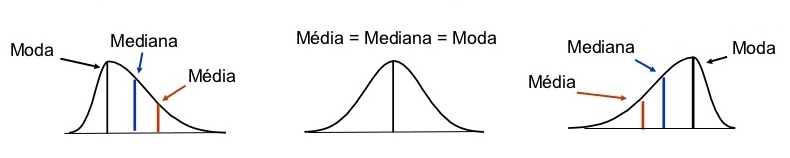
\includegraphics[width=0.9\linewidth]{./img/assimetria} 

}

\caption{Relação medidas descritivas e assimetria}\label{fig:unnamed-chunk-9}
\end{figure}
\end{frame}

\section{Medidas de posição
relativa}\label{medidas-de-posiuxe7uxe3o-relativa}

\begin{frame}{Medidas de posição relativa}
\phantomsection\label{medidas-de-posiuxe7uxe3o-relativa-1}
\beginAHalfColumn

\begin{itemize}
\tightlist
\item
  As medidas de posição relativa ou separatrizes buscam representar
  \textbf{pontos do domínio} em que a variável apresenta porções com
  frequências conhecidas.
\end{itemize}

\vspace{0.3cm}

\begin{itemize}
\tightlist
\item
  Visam encontrar valores que representam alguma parcela dos dados.
\end{itemize}

\endColumns
\beginAHalfColumn

\begin{itemize}
\tightlist
\item
  Algumas possiblidades são

  \begin{itemize}
  \tightlist
  \item
    Quartis.
  \item
    Decis.
  \item
    Percentis.
  \item
    Máximo.
  \item
    Mínimo.
  \end{itemize}
\end{itemize}

\endColumns
\end{frame}

\begin{frame}{Quartis}
\phantomsection\label{quartis}
\begin{itemize}
\tightlist
\item
  Dividem a amostra em \textbf{$4$ partes de mesmo tamanho}.
\item
  A ideia para obtenção é similar à da \textbf{mediana}.
\item
  Na verdade, a mediana é um dos quartis: o segundo.
\item
  O primeiro e terceiro quartil são as \textbf{medianas} das duas partes
  divididas pela mediana (método de Tukey).
\end{itemize}
\end{frame}

\begin{frame}{Quartis}
\phantomsection\label{quartis-1}
\begin{itemize}
\tightlist
\item
  O \textbf{primeiro quartil} (\(Q_1\)) é o valor que marca \(1/4\) das
  observações, isto é, \(25\%\).
\end{itemize}

\vspace{0.3cm}

\begin{itemize}
\tightlist
\item
  O \textbf{segundo quartil} (\(Q_2\)) é o valor que marca \(2/4=1/2\)
  das observações, isto é, \(50\%\) (a mediana).
\end{itemize}

\vspace{0.3cm}

\begin{itemize}
\tightlist
\item
  O \textbf{terceiro quartil} (\(Q_3\)) é o valor que marca \(3/4\) das
  observações, isto é, \(75\%\).
\end{itemize}

\vspace{0.3cm}

\begin{itemize}
\tightlist
\item
  A diferença entre primeiro e terceiro quartil é chamada de
  \textbf{amplitude interquartílica} (\(AIQ = Q_3-Q_1\)).
\end{itemize}

\vspace{0.3cm}

\begin{itemize}
\tightlist
\item
  Estas quantidades são usadas para criação de um poderoso gráfico: o
  \textbf{box-plot}.
\end{itemize}
\end{frame}

\begin{frame}{Quartis}
\phantomsection\label{quartis-2}
\textbf{Exemplo}

\begin{itemize}
\tightlist
\item
  Considere os seguintes valores:
\end{itemize}

\[6; 12; 14;  7; 11;  7;  6; 12;  4; 11;  3;  4;  3;  4;  2\]

\begin{itemize}
\item
  Obtenha os quartis e a amplitude interquartílica.
\item
  Passo 1: \textbf{ordenar}.
\end{itemize}

\begin{longtable}[]{@{}
  >{\raggedright\arraybackslash}p{(\linewidth - 30\tabcolsep) * \real{0.1356}}
  >{\centering\arraybackslash}p{(\linewidth - 30\tabcolsep) * \real{0.0508}}
  >{\centering\arraybackslash}p{(\linewidth - 30\tabcolsep) * \real{0.0508}}
  >{\centering\arraybackslash}p{(\linewidth - 30\tabcolsep) * \real{0.0508}}
  >{\centering\arraybackslash}p{(\linewidth - 30\tabcolsep) * \real{0.0508}}
  >{\centering\arraybackslash}p{(\linewidth - 30\tabcolsep) * \real{0.0508}}
  >{\centering\arraybackslash}p{(\linewidth - 30\tabcolsep) * \real{0.0508}}
  >{\centering\arraybackslash}p{(\linewidth - 30\tabcolsep) * \real{0.0508}}
  >{\centering\arraybackslash}p{(\linewidth - 30\tabcolsep) * \real{0.0508}}
  >{\centering\arraybackslash}p{(\linewidth - 30\tabcolsep) * \real{0.0508}}
  >{\centering\arraybackslash}p{(\linewidth - 30\tabcolsep) * \real{0.0678}}
  >{\centering\arraybackslash}p{(\linewidth - 30\tabcolsep) * \real{0.0678}}
  >{\centering\arraybackslash}p{(\linewidth - 30\tabcolsep) * \real{0.0678}}
  >{\centering\arraybackslash}p{(\linewidth - 30\tabcolsep) * \real{0.0678}}
  >{\centering\arraybackslash}p{(\linewidth - 30\tabcolsep) * \real{0.0678}}
  >{\centering\arraybackslash}p{(\linewidth - 30\tabcolsep) * \real{0.0678}}@{}}
\caption{Valores ordenados.}\tabularnewline
\toprule\noalign{}
\endfirsthead
\endhead
Posição & 1 & 2 & 3 & 4 & 5 & 6 & 7 & 8 & 9 & 10 & 11 & 12 & 13 & 14 &
15 \\
Valor & 2 & 3 & 3 & 4 & 4 & 4 & 6 & 6 & 7 & 7 & 11 & 11 & 12 & 12 &
14 \\
\bottomrule\noalign{}
\end{longtable}
\end{frame}

\begin{frame}{Quartis}
\phantomsection\label{quartis-3}
\beginAHalfColumn

\textbf{Exemplo}

\begin{itemize}
\tightlist
\item
  Passo 2: \textbf{obter o segundo quartil (mediana)}.

  \begin{itemize}
  \tightlist
  \item
    Número de elementos: \(15\).
  \item
    Posição do segundo quartil: \(8\).
  \item
    Valor do segundo quartil: \(6\).
  \end{itemize}
\item
  Passo 3: \textbf{obter a mediana dos valores da primeira parcela.}

  \begin{itemize}
  \tightlist
  \item
    Número de elementos: \(8\) (da posição 1 até 8).
  \item
    Posição da mediana da primeira parcela: \(4,5\).
  \item
    Valor do segundo quartil: \((4+4)/2 = 4\).
  \end{itemize}
\end{itemize}

\endColumns
\beginAHalfColumn

\begin{itemize}
\item
  Passo 4: \textbf{obter a mediana dos valores da segunda parcela.}

  \begin{itemize}
  \tightlist
  \item
    Número de elementos: \(8\) (da posição 8 até 15).
  \item
    Posição da mediana da segunda parcela: \(4,5\).
  \item
    Valor do segundo quartil: \((11+11)/2 = 11\).
  \end{itemize}
\item
  \(Q_1 = 4\), \(Q_2 = 6\), \(Q_3 = 11\).
\item
  Amplitude interquartílica.
\end{itemize}

\[AIQ = Q_3 - Q_1 = 11 - 4 = 7\]

\endColumns
\end{frame}

\begin{frame}{Quartis e o Box-plot}
\phantomsection\label{quartis-e-o-box-plot}
\begin{itemize}
\tightlist
\item
  O box-plot faz uso dos \textbf{quartis} para obtenção de um
  \textbf{gráfico}.
\item
  Com ele é possível analisar a distribuição dos dados:
  \textbf{posição}, \textbf{variabilidade}, \textbf{assimetria},
  \textbf{valores atípicos} (outliers).
\end{itemize}

\begin{figure}

{\centering 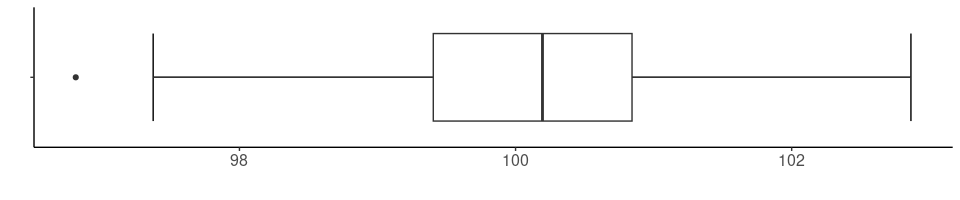
\includegraphics[width=0.9\linewidth]{./img/boxplot0} 

}

\caption{Ilustração box-plot completo.}\label{fig:unnamed-chunk-11}
\end{figure}
\end{frame}

\begin{frame}{Quartis e o Box-plot}
\phantomsection\label{quartis-e-o-box-plot-1}
\begin{itemize}
\item
  O Box-plot é construído a partir de \textbf{5 pontos} que resumem a
  distribuição dos dados observados: o \textbf{limite inferior}, o
  \textbf{1º quartil}, a \textbf{mediana}, o \textbf{3º quartil} e o
  \textbf{limite superior}.
\item
  Os \textbf{limites inferior} e \textbf{superior} são utilizados para
  detectar observações que estão longe da massa central localizada entre
  o primeiro e o terceiro quartis.
\item
  Entre o primeiro e terceiro quartil está a \textbf{mediana}. Não
  necessariamente a mediana estará no centro da caixa.
\end{itemize}

\begin{figure}

{\centering 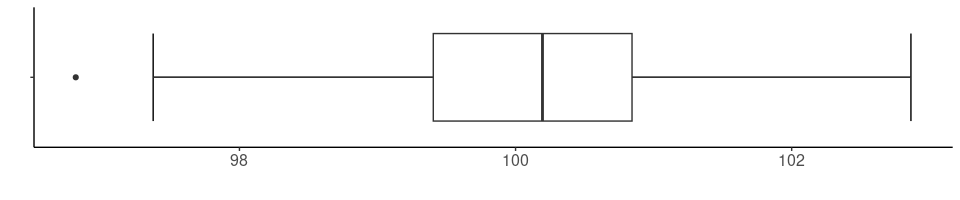
\includegraphics[width=0.9\linewidth]{./img/boxplot0} 

}

\caption{Ilustração box-plot completo.}\label{fig:unnamed-chunk-12}
\end{figure}
\end{frame}

\begin{frame}{Quartis e o Box-plot}
\phantomsection\label{quartis-e-o-box-plot-2}
\begin{itemize}
\tightlist
\item
  A construção de um box-plot inicia-se com um retângulo em que a aresta
  inferior coincide com o \textbf{primeiro quartil} e a superior com o
  \textbf{terceiro quartil}.
\end{itemize}

\begin{figure}

{\centering 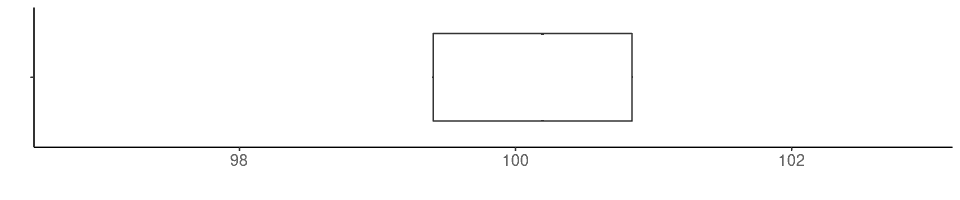
\includegraphics[width=0.9\linewidth]{./img/boxplot1} 

}

\caption{Arestas de um box-plot.}\label{fig:unnamed-chunk-13}
\end{figure}
\end{frame}

\begin{frame}{Quartis e o Box-plot}
\phantomsection\label{quartis-e-o-box-plot-3}
\begin{itemize}
\item
  A \textbf{mediana} é representada por um traço entre as duas arestas.
\item
  De \(Q_1\) até \(Q_3\) estão \(50\%\) das observações centrais, o que
  dá uma ideia a respeito de quão dispersos são os valores.
\end{itemize}

\begin{figure}

{\centering 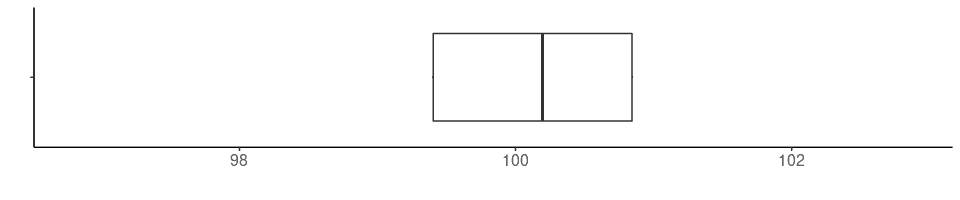
\includegraphics[width=0.9\linewidth]{./img/boxplot2} 

}

\caption{Arestas e mediana emum box-plot.}\label{fig:unnamed-chunk-14}
\end{figure}
\end{frame}

\begin{frame}{Quartis e o Box-plot}
\phantomsection\label{quartis-e-o-box-plot-4}
\begin{itemize}
\item
  Para obtenção da \textbf{amplitude do box-plot} além do retângulo
  faz-se \([Q1-1,5AIQ; Q3+1,5AIQ]\).
\item
  Desenha-se então uma linha até estes valores.

  \begin{itemize}
  \tightlist
  \item
    Se estes valores excedem o mínimo e o máximo da variável, então a
    linha para no mínimo e no máximo da variável.
  \end{itemize}
\end{itemize}

\begin{figure}

{\centering 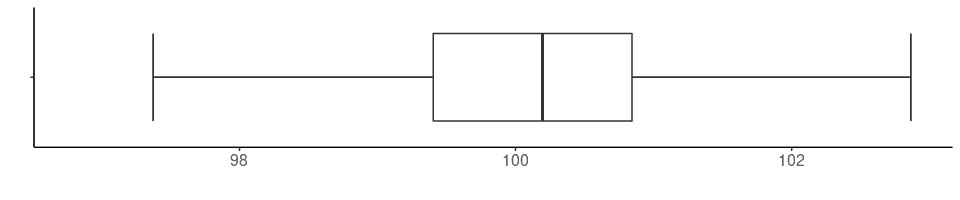
\includegraphics[width=0.9\linewidth]{./img/boxplot3} 

}

\caption{Inclusão dos limites de um box-plot.}\label{fig:unnamed-chunk-15}
\end{figure}
\end{frame}

\begin{frame}{Quartis e o Box-plot}
\phantomsection\label{quartis-e-o-box-plot-5}
\begin{itemize}
\tightlist
\item
  Valores além destes extremos são marcados como um ponto ou asterisco e
  são os candidatos a \textbf{valores atípicos}.
\end{itemize}

\begin{figure}

{\centering 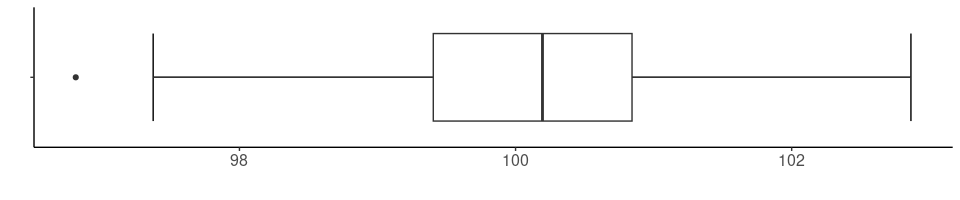
\includegraphics[width=0.9\linewidth]{./img/boxplot0} 

}

\caption{Box-plot completo.}\label{fig:unnamed-chunk-16}
\end{figure}
\end{frame}

\begin{frame}{Quartis e o Box-plot}
\phantomsection\label{quartis-e-o-box-plot-6}
\begin{itemize}
\item
  Os limitantes inferior e superior de um box-plot também são conhecidos
  como \textbf{valores adjacentes} ou também como
  \textbf{mínimo e máximo típicos}.
\item
  Existem outras formas de obtenção de um box-plot, como por exemplo o
  box-plot em que não são calculados o mínimo e máximo típicos.
\item
  Podem-se usar também outros quantis e outros pontos de corte, ou seja,
  existem outras formas para detectar pontos distantes da massa de
  dados.
\item
  A interpretação do gráfico vai depender de como ele foi construído.
\item
  Quanto mais observações, mais confiável será o box-plot.
\item
  Contudo, quanto mais observações é natural que surjam mais pontos além
  dos limites do gráfico.
\end{itemize}
\end{frame}

\begin{frame}{Quartis e o Box-plot}
\phantomsection\label{quartis-e-o-box-plot-7}
\begin{itemize}
\item
  Os pontos fora dos limites do box-plot costumam ser chamados de
  \textbf{valores atípicos ou outliers}.
\item
  A definição exata de outlier é bastante \textbf{subjetiva} e vai além
  dos box-plots.
\item
  Qualquer valor que seja muito distante dos outros valores em um
  conjunto de dados pode ser considerado outlier. Podemos usar o
  z-escore para verificar quais são os candidatos a outliers.
\item
  Ser um outlier não torna um valor inválido ou errado, mas é um
  indicativo de um comportamento atípico (que pode ser causado por um
  erro de medida por exemplo).
\end{itemize}
\end{frame}

\begin{frame}{Quartis para dados agrupados}
\phantomsection\label{quartis-para-dados-agrupados}
Para calcular os quartis quando os dados estão agrupados, considere:

\begin{itemize}
\tightlist
\item
  \(n\) é o número total de observações;
\item
  \(Q_i (i=1,2,3)\) é o quartil que desejamos obter;
\item
  \((i \cdot n/4)\) é a posição na qual se encontra o quartil \(Q_i\);
\item
  \(l\) é o limite inferior da classe que contem \(Q_i\);
\item
  \(f\) é a frequência na classe que contem \(Q_i\);
\item
  \(h\) é a amplitude na classe que contem \(Q_i\);
\item
  \(F_{ant}\) é a frequência acumulada até a classe anterior à que
  contem \(Q_i\).
\end{itemize}

O quartil \(Q_i\) é obtido aplicando-se a seguinte foŕmula:
\[Q_i=l+\frac{(i \cdot n/4-F_{ant})}{f} \cdot h\]
\end{frame}

\begin{frame}{Outras medidas}
\phantomsection\label{outras-medidas}
\begin{itemize}
\item
  O \textbf{mínimo} e o \textbf{máximo} também são medidas de posição
  relativa e fornecem informação quanto ao domínio da variável.
\item
  \textbf{Quartis} são a forma mais famosa de particionamento dos dados,
  porém qualquer outro percentual pode ser obtido.
\item
  Se temos um conjunto de \(n\) valores, organizados de forma crescente,
  o \(P\)-ésimo percentil é um número tal que \(P\%\) dos valores
  estejam à sua esquerda e \((100 - P)\%\) à sua direita.
\item
  Por exemplo, se obtivermos os valores que separam a amostra em \(10\)
  partes com frequência \(1/10\), temos os decis.
\item
  Estas \textbf{separatrizes} podem ser obtidas por meio do
  \textbf{gráfico de frequências acumuladas}.
\end{itemize}
\end{frame}

\section{Medidas de dispersão}\label{medidas-de-dispersuxe3o}

\begin{frame}{Medidas de dispersão}
\phantomsection\label{medidas-de-dispersuxe3o-1}
\begin{itemize}
\item
  Em geral usamos uma \textbf{medida de posição central}, que nos dá uma
  ideia de centro dos dados.
\item
  Mas conjuntos de dados com
  \textbf{diferentes valores podem gerar as mesmas medidas de posição}.
\item
  E mesmo com medidas de posição idênticas, um pode ser
  \textbf{mais disperso} que o outro.
\item
  Portanto \textbf{complementamos a informação} a respeito do centro
  \textbf{com uma medida de dispersão}, que nos dá uma noção de quão
  dispersos são os dados.
\end{itemize}
\end{frame}

\begin{frame}{Medidas de dispersão}
\phantomsection\label{medidas-de-dispersuxe3o-2}
Considere os seguintes conjuntos de valores:

\beginAHalfColumn

\begin{longtable}[]{@{}lrrrrrrrrrr@{}}
\toprule\noalign{}
\endhead
A & 5 & 5 & 5 & 5 & 5 & 5 & 5 & 5 & 5 & 5 \\
\bottomrule\noalign{}
\end{longtable}

\begin{longtable}[]{@{}lrrrrrrrrrr@{}}
\toprule\noalign{}
\endhead
B & 5 & 4 & 4 & 5 & 6 & 5 & 4 & 6 & 5 & 6 \\
\bottomrule\noalign{}
\end{longtable}

\begin{longtable}[]{@{}lrrrrrrrrrr@{}}
\toprule\noalign{}
\endhead
C & 0 & 5 & 9 & 0 & 5 & 11 & 10 & 5 & 5 & 0 \\
\bottomrule\noalign{}
\end{longtable}

\endColumns
\beginAHalfColumn

\begin{itemize}
\tightlist
\item
  Os conjuntos apresentam valores distintos, mas as medidas de posição
  central (média, moda e mediana), são idênticas.
\end{itemize}

\vspace{0.3cm}

\begin{itemize}
\tightlist
\item
  Precisamos de formas de mensurar o quanto os valores variam.
\end{itemize}

\endColumns
\end{frame}

\begin{frame}{Medidas de dispersão}
\phantomsection\label{medidas-de-dispersuxe3o-3}
\begin{itemize}
\item
  As medidas de dispersão são utilizadas para expressar informações como
  o \textbf{domínio} da variável, grau de \textbf{dispersão} ao redor do
  centro (\textbf{variabilidade}), e também \textbf{distanciamento} dos
  valores com relação ao centro.
\item
  Estas medidas buscam mensurar o quanto os dados estão ``compactados''
  ou ``espalhados''.
\item
  Uma medida de dispersão \textbf{não pode ser negativa}: ela será zero,
  indicando que todos os dados são iguais, ou ela é positiva, indicando
  algum grau de variabilidade nos dados.
\end{itemize}
\end{frame}

\begin{frame}{Medidas de dispersão}
\phantomsection\label{medidas-de-dispersuxe3o-4}
\begin{itemize}
\item
  As medidas de dispersão mais usadas são baseadas nas diferenças entre
  cada observação e uma medida de posição central, esta diferença é
  chamada de \textbf{desvio}.
\item
  Um jeito de medir a variabilidade como um todo é encontrar um
  \textbf{valor típico para os desvios}, como uma média.
\item
  Fazer isso com os desvios simples não é muito inteligente. Desvios
  negativos se anulam com os positivos e a soma dos desvios com relação
  a média sempre será 0.
\item
  Uma alternativa é calcular a média dos
  \textbf{desvios absolutos ou quadráticos} com relação a alguma medida
  de posição central.
\end{itemize}
\end{frame}

\begin{frame}{Medidas de dispersão}
\phantomsection\label{medidas-de-dispersuxe3o-5}
\begin{itemize}
\tightlist
\item
  Algumas medidas possíveis são

  \begin{itemize}
  \tightlist
  \item
    Amplitude.
  \item
    Desvio absluto médio ou mediano.
  \item
    Variância.
  \item
    Desvio padrão.
  \item
    Coeficiente de variação.
  \end{itemize}
\end{itemize}
\end{frame}

\begin{frame}{Amplitude}
\phantomsection\label{amplitude}
\begin{itemize}
\tightlist
\item
  Diferença entre o \textbf{maior} e o \textbf{menor} valor da variável.
\item
  Sensível a valores extremos.
\item
  Usa apenas duas medidas.
\end{itemize}

\[Amp = max(y) - min(y) = y(n) - y(1)\]
\end{frame}

\begin{frame}{Amplitude}
\phantomsection\label{amplitude-1}
\textbf{Exemplo}

\begin{itemize}
\tightlist
\item
  Retomando o problema das notas de 10 alunos, em que as notas obtidas
  foram:
\end{itemize}

\[60;\ 65;\ 77;\ 95;\ 56;\ 94;\ 97;\ 81;\ 80;\ 48\]

\[Y: \text{Notas obtidas.}\]

\[Amp = 97 - 48  = 49\]
\end{frame}

\begin{frame}{Desvio absoluto médio}
\phantomsection\label{desvio-absoluto-muxe9dio}
\begin{itemize}
\tightlist
\item
  Tomamos todos os \textbf{desvios absolutos} com relação a alguma
  medida de posição central (média ou mediana).
\item
  Calculamos a \textbf{média} destes desvios.
\item
  Uma medida alternativa é o \textbf{desvio absoluto mediano} em que em
  vez de calcular a média dos desvios absolutos calculamos a mediana.
\end{itemize}

\vspace{1cm}

\beginAHalfColumn

\[
DAM_{MÉDIA} = \frac{1}{n}
      \sum_{i = 1}^n |(y_i - \overline{y})|
\]

\endColumns
\beginAHalfColumn

\[
DAM_{MEDIANA} =
      \frac{1}{n} \sum_{i = 1}^n |(y_i - md)|
\]

\endColumns
\end{frame}

\begin{frame}{Desvio absoluto médio}
\phantomsection\label{desvio-absoluto-muxe9dio-1}
\textbf{Exemplo}

\begin{itemize}
\tightlist
\item
  Retomando o problema das notas de 10 alunos, em que as notas obtidas
  foram:
\end{itemize}

\[60;\ 65;\ 77;\ 95;\ 56;\ 94;\ 97;\ 81;\ 80;\ 48\]

\begin{itemize}
\item
  A média é \(\overline{y} = 75,3\) e a mediana é \(md = 78,5\).
\item
  Obtenha o desvio absoluto médio com relação à média e à mediana.
\end{itemize}
\end{frame}

\begin{frame}{Desvio absoluto médio}
\phantomsection\label{desvio-absoluto-muxe9dio-2}
\textbf{Exemplo - desvio absoluto médio com relação à média}

\[
DAM = \frac{1}{10}
       \left ( |(60 - 75,3)| + |(65 - 75,3)| ... + |(80 - 75,3)| + |(48 - 75,3)| \right )
\] \[
DAM = \frac{1}{10}
       \left ( 15,3 + 10,3 ... + 4,7  + 27,3  \right ) = 14,44
\]
\end{frame}

\begin{frame}{Desvio absoluto médio}
\phantomsection\label{desvio-absoluto-muxe9dio-3}
\textbf{Exemplo - desvio absoluto médio com relação à mediana}

\[
DAM = \frac{1}{10}
       \left ( |(60 - 78,5)| + |(65 - 78,5)| ... + |(80 - 78,5)| + |(48 - 78,5)| \right )
\] \[
DAM = \frac{1}{10}
       \left ( 18,5 + 13,5 ... + 1,5  + 30,5  \right ) = 14,1
\]
\end{frame}

\begin{frame}{Variância}
\phantomsection\label{variuxe2ncia}
\begin{itemize}
\tightlist
\item
  Em vez dos desvios, usa a \textbf{soma dos quadrados dos desvios} em
  relação à média.
\end{itemize}

\[
s^2 = \textrm{Var}(y) = \frac{1}{n - 1} \sum_{i = 1}^{n} (y_i - \overline{y})^2 = \frac{1}{n - 1}\left(\sum_{i = 1}^{n} y_i^2 - \frac{(\sum_{i = 1}^{n} y_i)^2}{n}\right)
\]

\begin{itemize}
\item
  A \textbf{variância populacional} (\(\sigma^2\)): usa apenas \(n\) no
  demominador e é usada quando temos todos os elementos da população.
  Caso contrário, calculamos sempre a estimativa \textbf{amostral}
  (\(s^2\)).
\item
  A justificativa teórica para isso está relacionada com
  \textbf{estimadores não viciados} e com a
  \textbf{distribuição amostral da média}, tópicos discutidos em
  inferência estatística.
\end{itemize}
\end{frame}

\begin{frame}{Desvio padrão}
\phantomsection\label{desvio-padruxe3o}
\begin{itemize}
\tightlist
\item
  Para ter uma medida de dispersão com a
  \textbf{mesma unidade de medida dos dados originais} definiu-se o
  \textbf{desvio padrão} como a raiz quadrada da variância.
\end{itemize}

\[
s = \sqrt{s^2}
\]

\begin{itemize}
\tightlist
\item
  A \textbf{variância} e o \textbf{desvio padrão} são
  \textbf{invariantes} com respeito a localização dos dados. Isso
  significa que, se somarmos ou subtrairmos uma constante em todos os
  valores, não alteramos a dispersão.
\end{itemize}
\end{frame}

\begin{frame}{Lei de Chebyshev}
\phantomsection\label{lei-de-chebyshev}
\begin{itemize}
\item
  Independente da forma da distribuição dos dados e de sua
  variabilidade, conhecemos a
  \textbf{proporção mínima dos valores contidos em intervalos simétricos em relação à média}:

  \begin{itemize}
  \item
    Pelo menos \(3/4\) (\(75\%\)) dos valores estão no intervalo
    \((\bar{y} - 2s, \bar{y} + 2s)\).
  \item
    Pelo menos \(8/9\) (\(89\%\)) dos valores estão no intervalo
    \((\bar{y} - 3s, \bar{y} + 3s)\).
  \item
    Pelos menos (\(1 - 1/k^2\)) dos dados estará no intervalo
    \((\bar{y} - ks, \bar{y} + ks)\).
  \end{itemize}
\end{itemize}
\end{frame}

\begin{frame}{Variância e desvio padrão}
\phantomsection\label{variuxe2ncia-e-desvio-padruxe3o}
\textbf{Exemplo}

\begin{itemize}
\tightlist
\item
  Retomando o problema das notas de 10 alunos, em que as notas obtidas
  foram:
\end{itemize}

\[60;\ 65;\ 77;\ 95;\ 56;\ 94;\ 97;\ 81;\ 80;\ 48\]

\begin{itemize}
\item
  A média é \(\overline{y} = 75,3\).
\item
  Obtenha o variância e desvio padrão.
\end{itemize}
\end{frame}

\begin{frame}{Variância e desvio padrão}
\phantomsection\label{variuxe2ncia-e-desvio-padruxe3o-1}
\textbf{Exemplo}

\begin{itemize}
\tightlist
\item
  Primeira maneira:
\end{itemize}

\[
s^2 = \textrm{Var}(y) = \frac{1}{10 - 1} \left ( (60 - 75,3)^2 + (65 - 75,3)^2 + ... + (80 - 75,3)^2 + (48 - 75,3)^2   \right )
\]

\[
s^2 = \textrm{Var}(y) = \frac{1}{9} \left ( (-15,3)^2 + (-10,3)^2 + ... + (4,7)^2 + (-27,3)^2   \right )
\]

\[
s^2 = \textrm{Var}(y) = \frac{1}{9} \left ( 234,09 + 106,09 + ... + 22,09 + 745,29 \right ) = 302,68
\]

\[ s = \sqrt{s^2} = \sqrt{302,68} = 17,4\]
\end{frame}

\begin{frame}{Variância e desvio padrão}
\phantomsection\label{variuxe2ncia-e-desvio-padruxe3o-2}
\textbf{Exemplo}

\begin{itemize}
\tightlist
\item
  Segunda maneira:
\end{itemize}

\[
s^2 = \textrm{Var}(y) = \frac{1}{n - 1}\left(\sum_{i = 1}^{n} y_i^2 - \frac{(\sum_{i = 1}^{n} y_i)^2}{n}\right)
\]

\[
s^2 = \textrm{Var}(y) = \frac{1}{9}\left(59425
 - \frac{753^2}{10}\right) = \frac{1}{9}\left(59425
 - 56700.9\right) = 302,68
\]

\[ s = \sqrt{s^2} = \sqrt{302,68} = 17,4\]
\end{frame}

\begin{frame}{Coeficiente de variação}
\phantomsection\label{coeficiente-de-variauxe7uxe3o}
\begin{itemize}
\tightlist
\item
  Medida de variabilidade relativa à média.
\item
  Quociente do desvio-padrão pela média.
\item
  \textbf{Medida adimensional}, geralmente apresentada na forma de
  porcentagem.
\item
  Permite comparar a variabilidade de variáveis de diferentes naturezas
\end{itemize}

\[
\textrm{CV} = 100 \cdot \frac{s}{\overline{y}}
\]
\end{frame}

\begin{frame}{Coeficiente de variação}
\phantomsection\label{coeficiente-de-variauxe7uxe3o-1}
\textbf{Exemplo}

\begin{itemize}
\tightlist
\item
  Retomando o problema das notas de 10 alunos, em que as notas obtidas
  foram:
\end{itemize}

\[60;\ 65;\ 77;\ 95;\ 56;\ 94;\ 97;\ 81;\ 80;\ 48\]

\begin{itemize}
\item
  A média é \(\overline{y} = 75,3\) e o desvio padrão é \(s = 17,4\).
\item
  Obtenha o coeficiente de variação.
\end{itemize}

\[
\textrm{CV} = 100 \cdot \frac{17,4}{75,3} = 23,11
\]
\end{frame}

\begin{frame}{z-escore}
\phantomsection\label{z-escore}
\begin{itemize}
\item
  O z-escore pode ser visto como uma
  \textbf{medida de variabilidade individual} que nos diz quantos
  desvios padrões determinada observação está distante da média dos
  dados.
\item
  O z-escore é dado por:
\end{itemize}

\[z = \frac{y_i-\bar{y}}{s}\]
\end{frame}

\begin{frame}{z-escore}
\phantomsection\label{z-escore-1}
\textbf{Exemplo}

\begin{itemize}
\tightlist
\item
  No problema das notas de 10 alunos, em que as notas obtidas foram:
\end{itemize}

\[60;\ 65;\ 77;\ 95;\ 56;\ 94;\ 97;\ 81;\ 80;\ 48\]

os z-escores para cada nota seriam:

\[-0,8794;\ -0,5920;\  0,0977;\  1,1323;\ -1,1093;\  1,0749;\  1,2473;\  0,3276;\  0,2702;\ -1,5692\]
\end{frame}

\begin{frame}{Dispersão para variáveis qualitativas}
\phantomsection\label{dispersuxe3o-para-variuxe1veis-qualitativas}
\begin{itemize}
\item
  Para variáveis qualitativas a \textbf{moda} é a única medida de
  posição que faz sentido.
\item
  Como medida de dispersão, a ideia de \textbf{entropia} pode ser usada.
\item
  Uma proposta, chamada de \textbf{índice de Shannon}, é dada por:
\end{itemize}

\[H = - \sum_{i=1}^{S} f_r ln(f_r)\]

\begin{itemize}
\item
  Em que \(S\) representa o número de categorias da variável e \(f_r\)
  representa a frequência relativa associada à categoria \(i\).
\item
  Quanto mais distante de \(0\) for o valor de \(H\), mais heterogênea é
  a variável.
\end{itemize}
\end{frame}

\begin{frame}{Dispersão para variáveis qualitativas}
\phantomsection\label{dispersuxe3o-para-variuxe1veis-qualitativas-1}
Qual é o mais homogêneo? Qual é o mais heterogêneo?

\begin{center}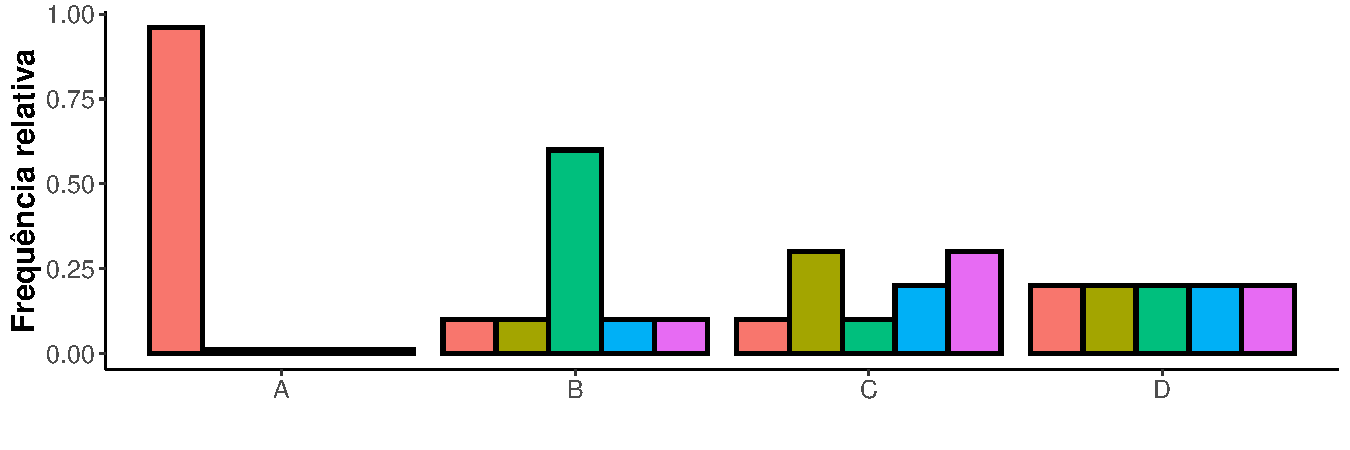
\includegraphics[width=11cm]{encontro2_files/figure-beamer/unnamed-chunk-18-1} \end{center}

\begin{longtable}[]{@{}lrrrrr@{}}
\toprule\noalign{}
& \(f_{r1}\) & \(f_{r2}\) & \(f_{r3}\) & \(f_{r4}\) & \(f_{r5}\) \\
\midrule\noalign{}
\endhead
A & 0.96 & 0.01 & 0.01 & 0.01 & 0.01 \\
B & 0.10 & 0.10 & 0.60 & 0.10 & 0.10 \\
C & 0.10 & 0.30 & 0.10 & 0.20 & 0.30 \\
D & 0.20 & 0.20 & 0.20 & 0.20 & 0.20 \\
\bottomrule\noalign{}
\end{longtable}
\end{frame}

\begin{frame}{Dispersão para variáveis qualitativas}
\phantomsection\label{dispersuxe3o-para-variuxe1veis-qualitativas-2}
Qual é o mais homogêneo? Qual é o mais heterogêneo?

\begin{center}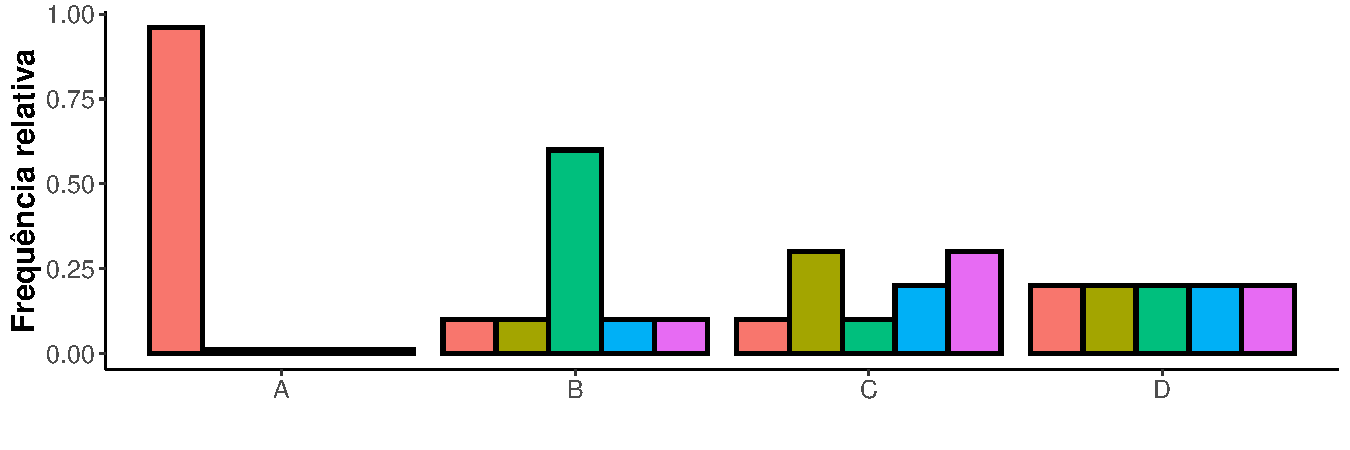
\includegraphics[width=11cm]{encontro2_files/figure-beamer/unnamed-chunk-19-1} \end{center}

\begin{longtable}[]{@{}lrrrrrr@{}}
\toprule\noalign{}
& \(f_{r1}\) & \(f_{r2}\) & \(f_{r3}\) & \(f_{r4}\) & \(f_{r5}\) & H \\
\midrule\noalign{}
\endhead
A & 0.96 & 0.01 & 0.01 & 0.01 & 0.01 & 0.223 \\
B & 0.10 & 0.10 & 0.60 & 0.10 & 0.10 & 1.228 \\
C & 0.10 & 0.30 & 0.10 & 0.20 & 0.30 & 1.505 \\
D & 0.20 & 0.20 & 0.20 & 0.20 & 0.20 & 1.609 \\
\bottomrule\noalign{}
\end{longtable}
\end{frame}

\begin{frame}{Desvio, variância, desvio padrão, coeficiente de variação,
entropia}
\phantomsection\label{desvio-variuxe2ncia-desvio-padruxe3o-coeficiente-de-variauxe7uxe3o-entropia}
\begin{itemize}
\item
  Amplitude, desvio absoluto médio, variância e desvio padrão são
  \textbf{sensíveis a valores extremos}. Variância e desvio padrão ainda
  mais por serem baseados nos desvios quadráticos.
\item
  \textbf{Variância} e \textbf{desvio padrão} tem
  \textbf{propriedades favoráveis}.
\item
  O \textbf{desvio absoluto mediano da mediana} é uma medida que
  \textbf{não é influenciada}, assim como variâncias e desvios padrões
  aparados.
\item
  Quando a distribuição dos dados é \textbf{simétrica} estas medidas
  tendem a convergir.
\item
  O \textbf{coeficiente de variação} permite comparar a variabilidade de
  variáveis em \textbf{diferentes escalas}.
\item
  O \textbf{z-escore} pode ser usado como uma medida de
  \textbf{variabilidade individual}.
\item
  Para \textbf{variáveis qualitativas} existem medidas específicas, como
  o \textbf{índice de Shannon}.
\end{itemize}
\end{frame}

\section{Análise exploratória
bivariada}\label{anuxe1lise-exploratuxf3ria-bivariada}

\begin{frame}{Análise exploratória bivariada}
\phantomsection\label{anuxe1lise-exploratuxf3ria-bivariada-1}
\beginAHalfColumn

\begin{itemize}
\tightlist
\item
  Em alguns casos podemos estar interessados na análise de
  \textbf{duas variáveis simultaneamente}.
\end{itemize}

\vspace{0.3cm}

\begin{itemize}
\tightlist
\item
  O objetivo é investigar a relação de \textbf{associação} entre as
  variáveis.
\end{itemize}

\vspace{0.3cm}

\begin{itemize}
\tightlist
\item
  \textbf{Tabelas}, \textbf{gráficos} e \textbf{coeficientes}
  específicos para relação entre variáveis podem ser usados.
\end{itemize}

\endColumns
\beginAHalfColumn

\begin{itemize}
\tightlist
\item
  Tal como nas análises univariadas, as escolhas dependem dos tipos das
  variáveis.
\end{itemize}

\vspace{0.3 cm}

\begin{itemize}
\tightlist
\item
  Considerando variáveis aos pares, as combinações podem ser:

  \begin{itemize}
  \tightlist
  \item
    Qualitativa x qualitativa.
  \item
    Quantitativa x quantitativa.
  \item
    Quantitativa x qualitativa.
  \end{itemize}
\end{itemize}

\endColumns
\end{frame}

\section{Análise bivariada para variáveis
qualitativas}\label{anuxe1lise-bivariada-para-variuxe1veis-qualitativas}

\begin{frame}{Análise bivariada para variáveis qualitativas}
\phantomsection\label{anuxe1lise-bivariada-para-variuxe1veis-qualitativas-1}
\begin{itemize}
\item
  Neste tipo de situação avaliamos a \textbf{frequência} de observações
  para cada \textbf{combinação} de níveis das duas variáveis.
\item
  Podem ser usadas \textbf{tabelas de frequências cruzadas}, também
  chamadas de \textbf{tabelas de dupla entrada}.
\item
  Também é possível representar as frequências por meio de
  \textbf{recursos gráficos}.
\end{itemize}
\end{frame}

\begin{frame}{Tabelas de frequências cruzadas}
\phantomsection\label{tabelas-de-frequuxeancias-cruzadas}
\begin{itemize}
\tightlist
\item
  As \textbf{linhas} dizem respeito aos \textbf{níveis} de uma variável.
\item
  As \textbf{colunas} aos \textbf{níveis} da outra variável.
\item
  As \textbf{células} mostram as \textbf{frequências} (absolutas ou
  relativas).
\item
  As tabelas de dupla entrada também são chamadas de
  \textbf{distribuição conjunta}.
\item
  As \textbf{margens} mostram as \textbf{frequências marginais} (de
  apenas uma das duas variáveis), também chamada de
  \textbf{distribuição marginal}.
\item
  No caso de frequências relativas podem ser usados o
  \textbf{total geral} ou os totais \textbf{linha} e \textbf{coluna}.
\end{itemize}
\end{frame}

\begin{frame}{Tabelas de frequências cruzadas}
\phantomsection\label{tabelas-de-frequuxeancias-cruzadas-1}
\begin{longtable}[]{@{}lcccc@{}}
\caption{Tabela de dupla entrada usando frequências
absolutas.}\tabularnewline
\toprule\noalign{}
& capital & interior & outro & Total \\
\midrule\noalign{}
\endfirsthead
\toprule\noalign{}
& capital & interior & outro & Total \\
\midrule\noalign{}
\endhead
casado & 7 & 8 & 5 & 20 \\
solteiro & 4 & 4 & 8 & 16 \\
Total & 11 & 12 & 13 & 36 \\
\bottomrule\noalign{}
\end{longtable}
\end{frame}

\begin{frame}{Tabelas de frequências cruzadas}
\phantomsection\label{tabelas-de-frequuxeancias-cruzadas-2}
\begin{longtable}[]{@{}lcccc@{}}
\caption{Tabela de dupla entrada usando frequências
relativas.}\tabularnewline
\toprule\noalign{}
& capital & interior & outro & Total \\
\midrule\noalign{}
\endfirsthead
\toprule\noalign{}
& capital & interior & outro & Total \\
\midrule\noalign{}
\endhead
casado & 0.19 & 0.22 & 0.14 & 0.56 \\
solteiro & 0.11 & 0.11 & 0.22 & 0.44 \\
Total & 0.31 & 0.33 & 0.36 & 1.00 \\
\bottomrule\noalign{}
\end{longtable}
\end{frame}

\begin{frame}{Tabelas de frequências cruzadas}
\phantomsection\label{tabelas-de-frequuxeancias-cruzadas-3}
\begin{longtable}[]{@{}lcccc@{}}
\caption{Tabela de dupla entrada usando frequências relativas aos totais
linha.}\tabularnewline
\toprule\noalign{}
& capital & interior & outro & Total \\
\midrule\noalign{}
\endfirsthead
\toprule\noalign{}
& capital & interior & outro & Total \\
\midrule\noalign{}
\endhead
casado & 0.35 & 0.40 & 0.25 & 1 \\
solteiro & 0.25 & 0.25 & 0.50 & 1 \\
Total & 0.31 & 0.33 & 0.36 & 1 \\
\bottomrule\noalign{}
\end{longtable}
\end{frame}

\begin{frame}{Tabelas de frequências cruzadas}
\phantomsection\label{tabelas-de-frequuxeancias-cruzadas-4}
\begin{longtable}[]{@{}lcccc@{}}
\caption{Tabela de dupla entrada usando frequências relativas aos totais
coluna.}\tabularnewline
\toprule\noalign{}
& capital & interior & outro & Total \\
\midrule\noalign{}
\endfirsthead
\toprule\noalign{}
& capital & interior & outro & Total \\
\midrule\noalign{}
\endhead
casado & 0.64 & 0.67 & 0.38 & 0.56 \\
solteiro & 0.36 & 0.33 & 0.62 & 0.44 \\
Total & 1.00 & 1.00 & 1.00 & 1.00 \\
\bottomrule\noalign{}
\end{longtable}
\end{frame}

\begin{frame}{Análise bivariada para variáveis qualitativas}
\phantomsection\label{anuxe1lise-bivariada-para-variuxe1veis-qualitativas-2}
\beginAHalfColumn

\begin{itemize}
\tightlist
\item
  As \textbf{frequências cruzadas} podem ser representadas por meio de
  gráficos.
\end{itemize}

\vspace{0.3cm}

\begin{itemize}
\tightlist
\item
  Variações de \textbf{gráficos de barras} são as opções mais comuns.
\end{itemize}

\vspace{0.3cm}

\begin{itemize}
\tightlist
\item
  As possibilidades podem usar as \textbf{frequências absolutas},
  \textbf{relativas} e permitem comparar a \textbf{composição} das
  variáveis.
\end{itemize}

\endColumns
\beginAHalfColumn

\begin{itemize}
\tightlist
\item
  Gráficos para frequência para duas variáveis qualitativas:

  \begin{itemize}
  \tightlist
  \item
    Gráficos de barras lado a lado.
  \item
    Gráfico de barras empilhadas.
  \item
    Gráficos de barras empilhadas relativo.
  \end{itemize}
\end{itemize}

\endColumns
\end{frame}

\begin{frame}{Gráficos de barras lado a lado}
\phantomsection\label{gruxe1ficos-de-barras-lado-a-lado}
\begin{figure}

{\centering 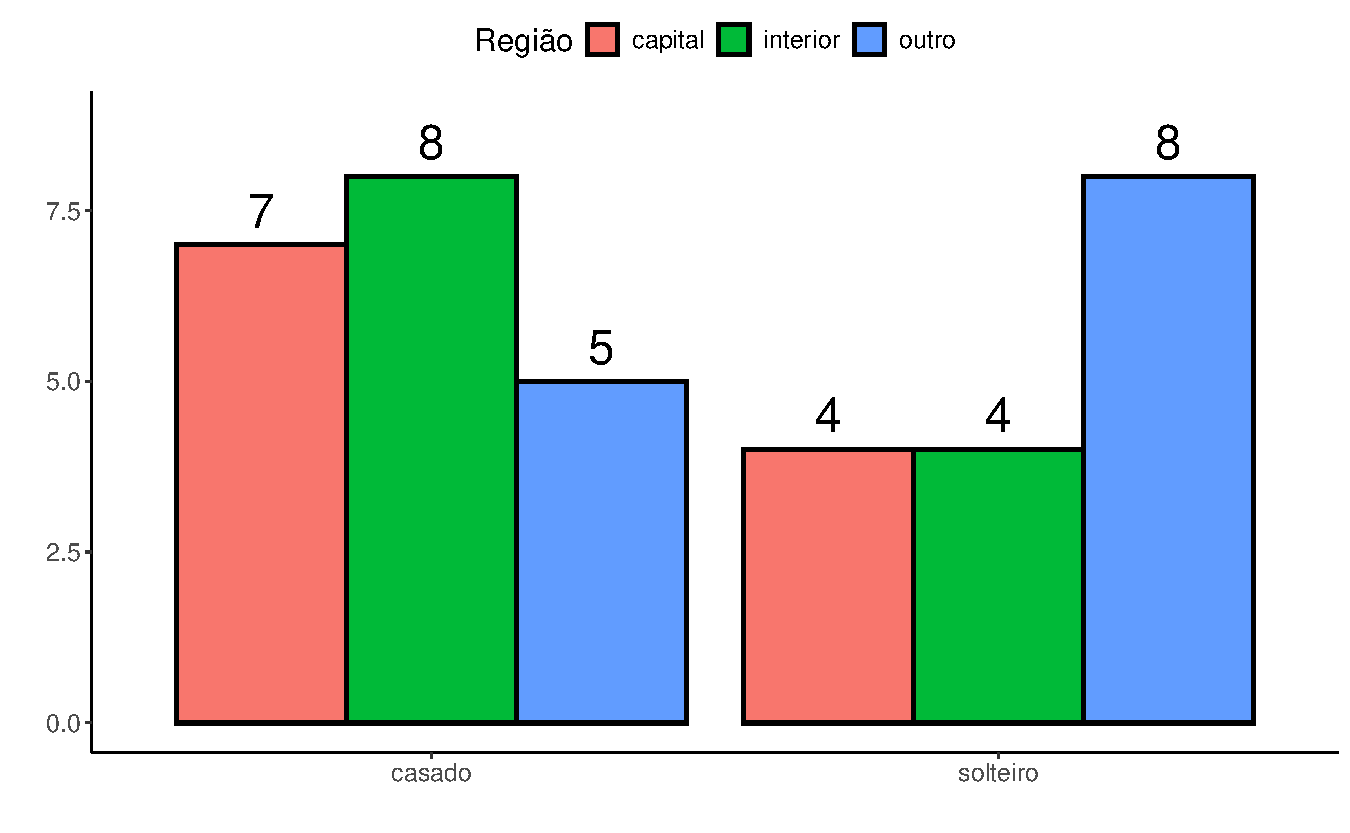
\includegraphics[width=11cm]{encontro2_files/figure-beamer/unnamed-chunk-24-1} 

}

\caption{Gráfico de barras lado a lado.}\label{fig:unnamed-chunk-24}
\end{figure}
\end{frame}

\begin{frame}{Gráficos de barras lado a lado}
\phantomsection\label{gruxe1ficos-de-barras-lado-a-lado-1}
\begin{figure}

{\centering 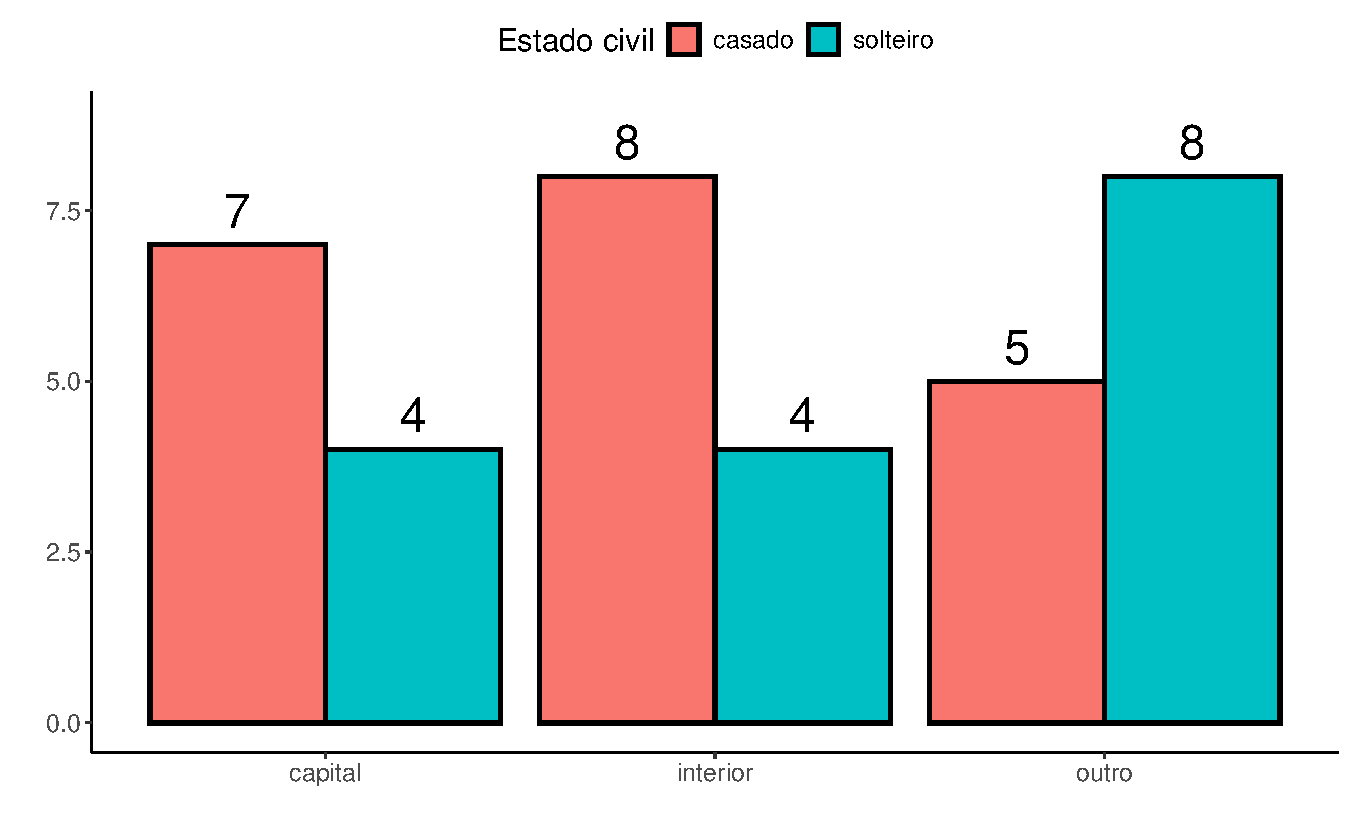
\includegraphics[width=11cm]{encontro2_files/figure-beamer/unnamed-chunk-25-1} 

}

\caption{Gráfico de barras lado a lado.}\label{fig:unnamed-chunk-25}
\end{figure}
\end{frame}

\begin{frame}{Gráficos de barras empilhadas}
\phantomsection\label{gruxe1ficos-de-barras-empilhadas}
\begin{figure}

{\centering 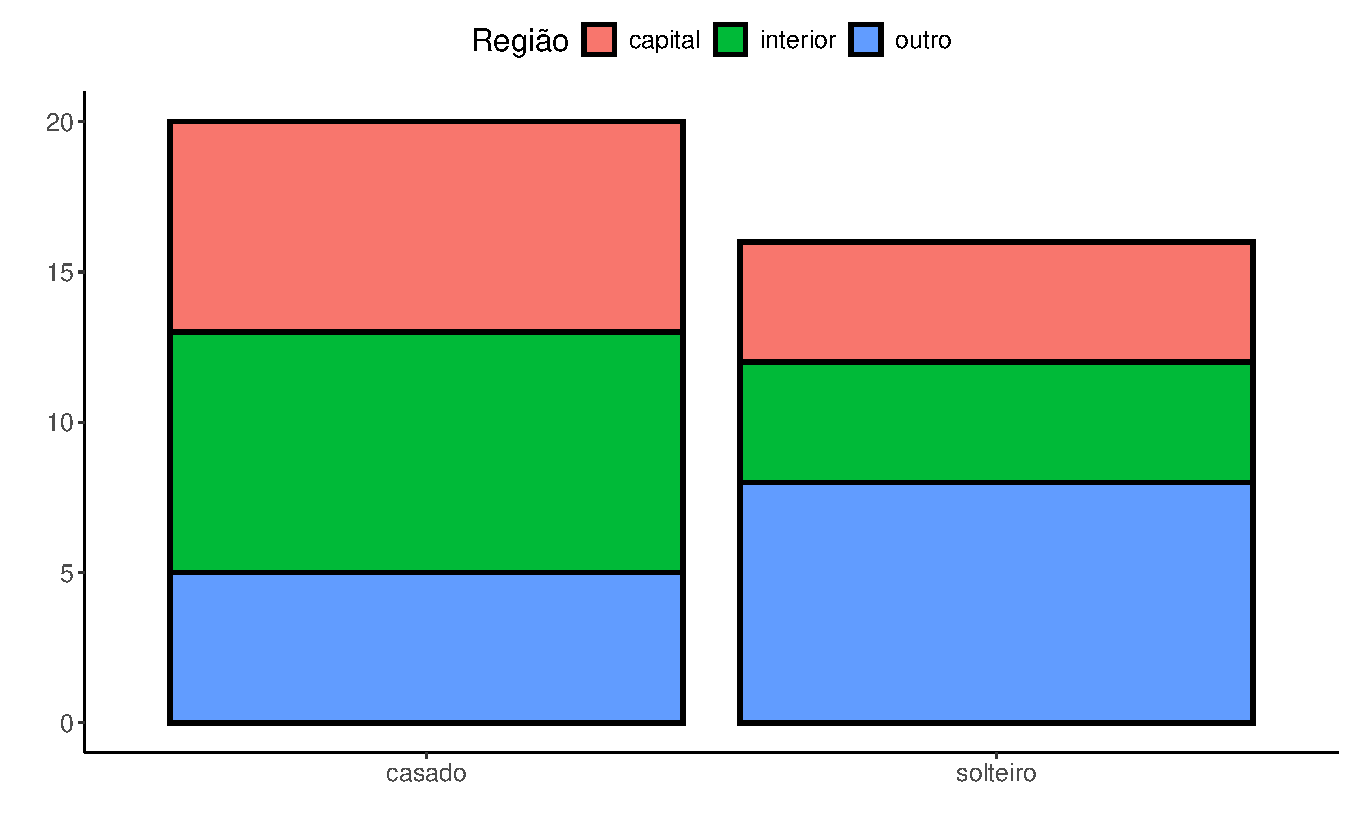
\includegraphics[width=11cm]{encontro2_files/figure-beamer/unnamed-chunk-26-1} 

}

\caption{Gráfico de barras empilhadas.}\label{fig:unnamed-chunk-26}
\end{figure}
\end{frame}

\begin{frame}{Gráficos de barras empilhadas}
\phantomsection\label{gruxe1ficos-de-barras-empilhadas-1}
\begin{figure}

{\centering 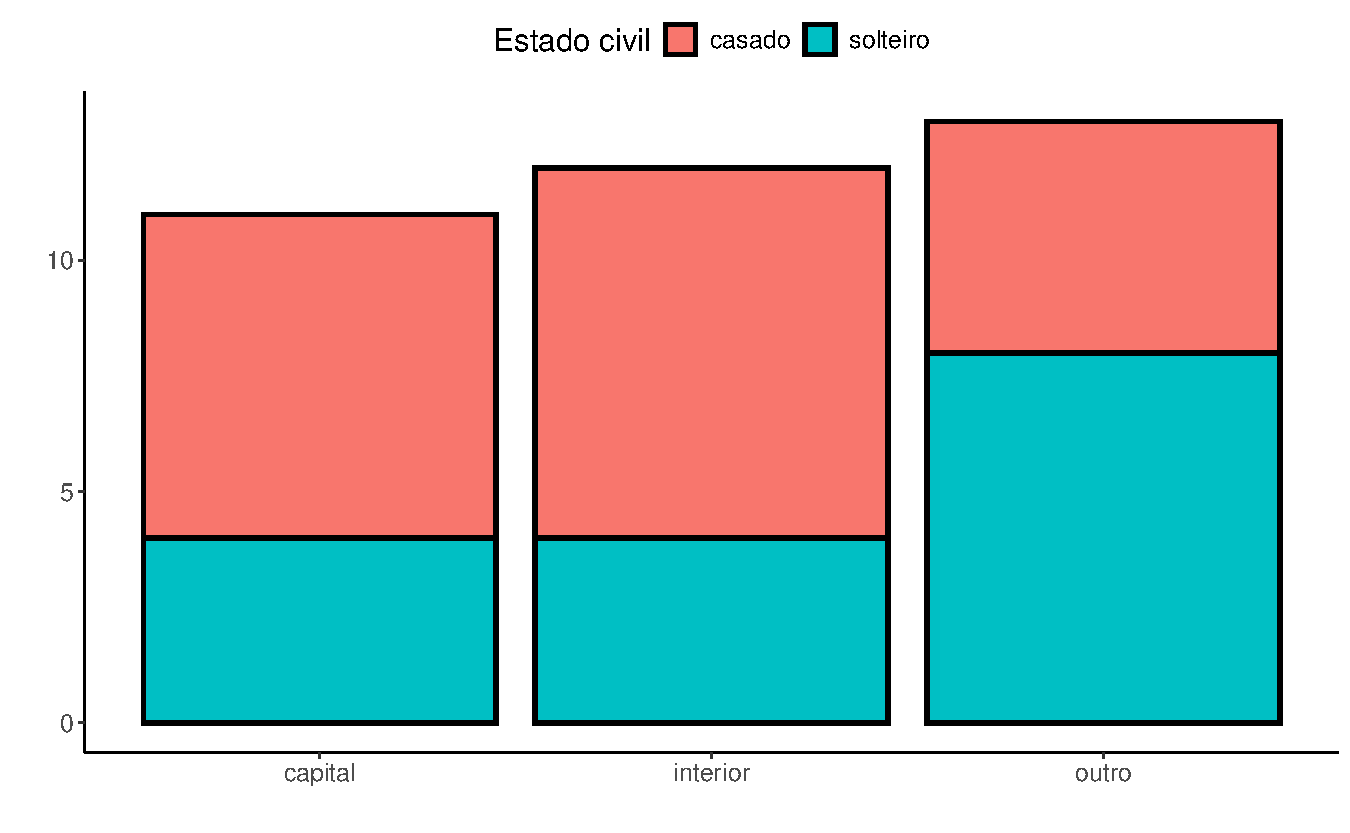
\includegraphics[width=11cm]{encontro2_files/figure-beamer/unnamed-chunk-27-1} 

}

\caption{Gráfico de barras empilhadas.}\label{fig:unnamed-chunk-27}
\end{figure}
\end{frame}

\begin{frame}{Gráficos de barras empilhadas relativo}
\phantomsection\label{gruxe1ficos-de-barras-empilhadas-relativo}
\begin{figure}

{\centering 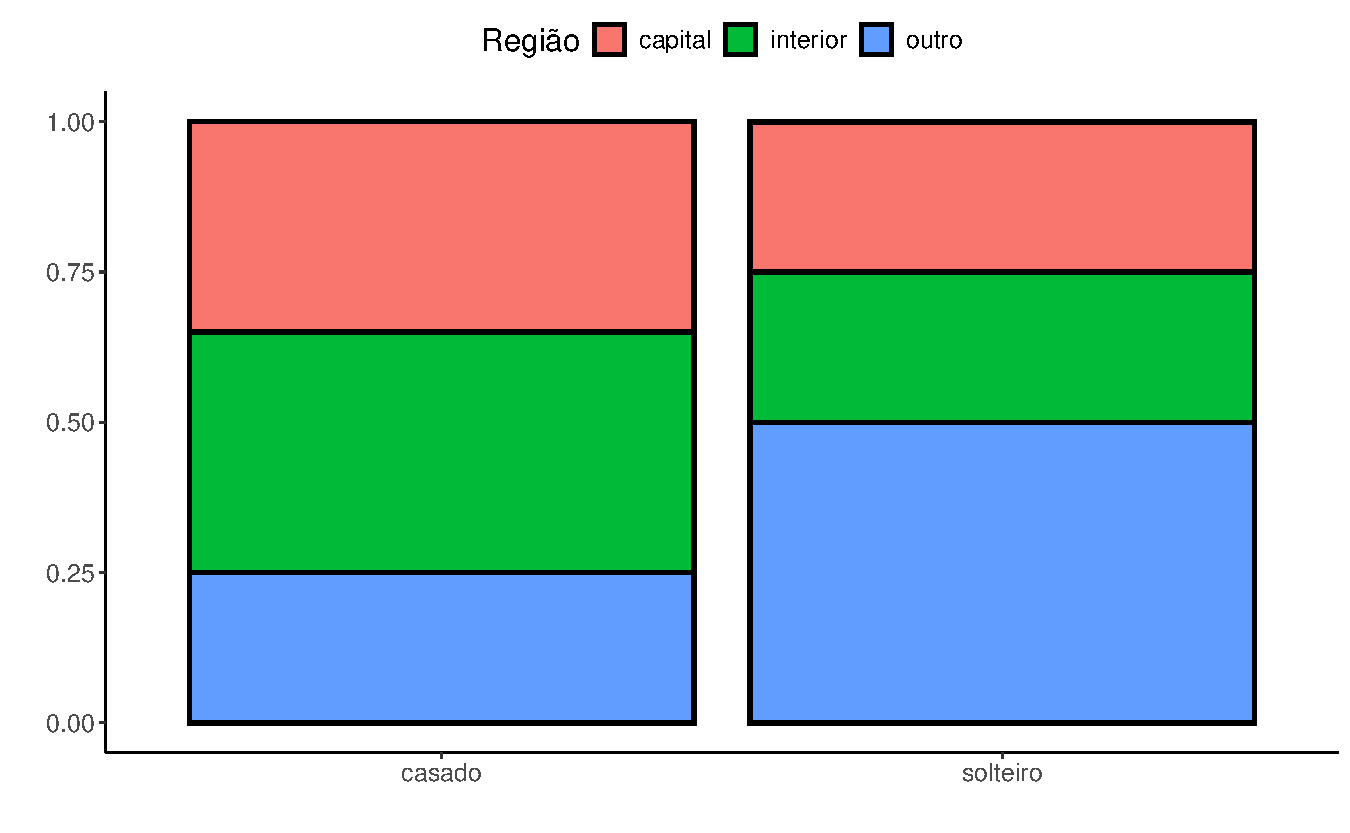
\includegraphics[width=11cm]{encontro2_files/figure-beamer/unnamed-chunk-28-1} 

}

\caption{Gráfico de barras empilhadas relativo.}\label{fig:unnamed-chunk-28}
\end{figure}
\end{frame}

\begin{frame}{Gráficos de barras empilhadas relativo}
\phantomsection\label{gruxe1ficos-de-barras-empilhadas-relativo-1}
\begin{figure}

{\centering 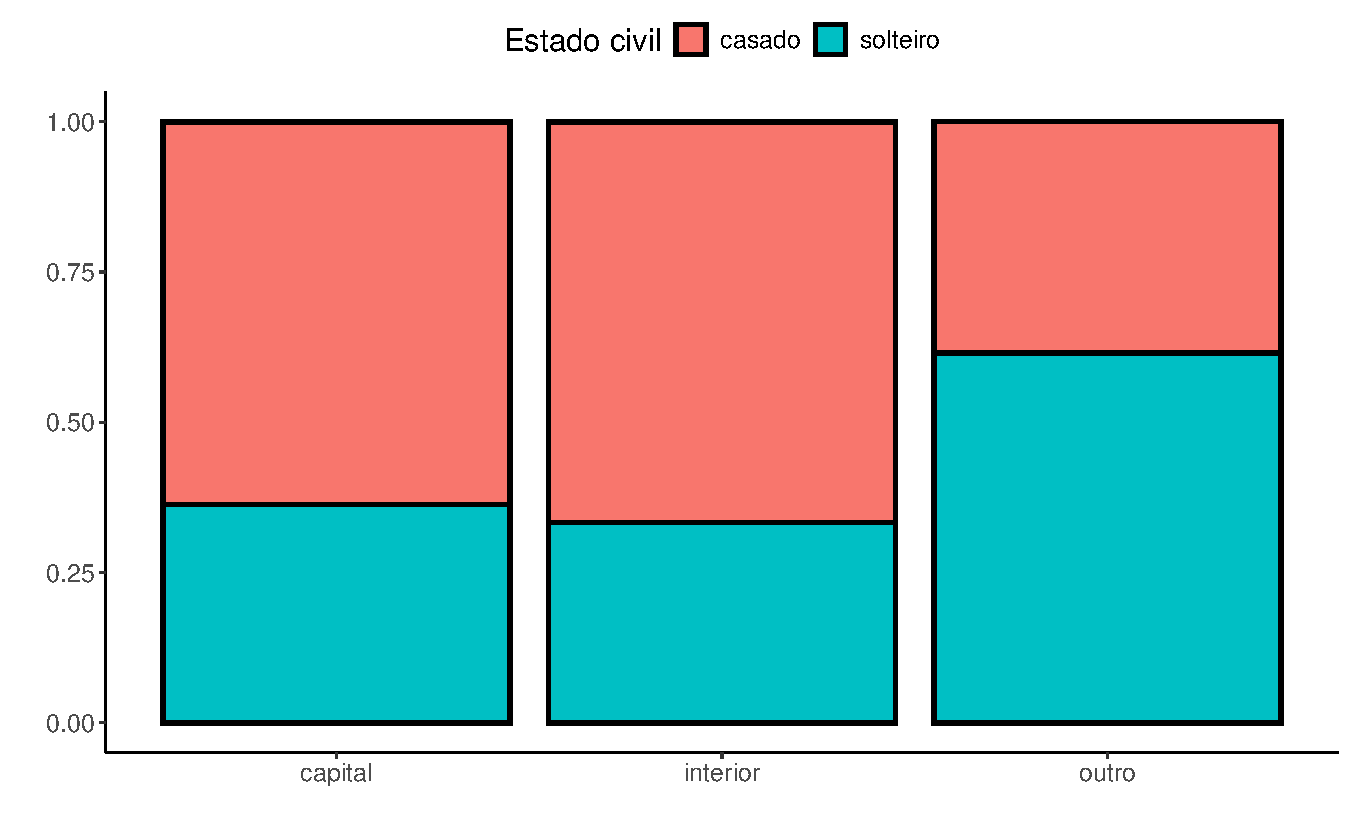
\includegraphics[width=11cm]{encontro2_files/figure-beamer/unnamed-chunk-29-1} 

}

\caption{Gráfico de barras empilhadas relativo.}\label{fig:unnamed-chunk-29}
\end{figure}
\end{frame}

\begin{frame}{Medidas de associação para variáveis qualitativas}
\phantomsection\label{medidas-de-associauxe7uxe3o-para-variuxe1veis-qualitativas}
\begin{itemize}
\item
  Existem \textbf{medidas} que visam quantificar o
  \textbf{grau de associação} entre variáveis qualitativas.
\item
  Uma dessas medidas é chamada de \textbf{Qui-quadrado}.
\item
  Esta medida compara as \textbf{frequências observadas} em uma tabela
  de dupla entrada com as \textbf{frequências esperadas} caso não
  houvesse associação.
\item
  Para obter a tabela de valores esperados basta, para cada casela,
  obter o produto entre o total da respectiva linha pelo total da
  respectiva coluna e dividir pelo total geral.
\end{itemize}
\end{frame}

\begin{frame}{Medidas de associação para variáveis qualitativas}
\phantomsection\label{medidas-de-associauxe7uxe3o-para-variuxe1veis-qualitativas-1}
\begin{itemize}
\tightlist
\item
  O qui-quadrado é dado por:
\end{itemize}

\[Q = \sum_{i=1}^{r} \sum_{j=1}^{s} \frac{(o_{ij} - e_{ij})^2}{e_{ij}}\]

\begin{itemize}
\item
  Quanto mais próximo de 0, menor a evidência de associação.
\item
  Como o valor é irrestrito, existem variações desta quantidade que
  visam ter os limites definidos.
\end{itemize}
\end{frame}

\begin{frame}{Medidas de associação para variáveis qualitativas}
\phantomsection\label{medidas-de-associauxe7uxe3o-para-variuxe1veis-qualitativas-2}
\begin{longtable}[]{@{}lcccc@{}}
\caption{Valores observados.}\tabularnewline
\toprule\noalign{}
& capital & interior & outro & Total \\
\midrule\noalign{}
\endfirsthead
\toprule\noalign{}
& capital & interior & outro & Total \\
\midrule\noalign{}
\endhead
casado & 7 & 8 & 5 & 20 \\
solteiro & 4 & 4 & 8 & 16 \\
Total & 11 & 12 & 13 & 36 \\
\bottomrule\noalign{}
\end{longtable}

\begin{longtable}[]{@{}lcccc@{}}
\caption{Valores esperados.}\tabularnewline
\toprule\noalign{}
& capital & interior & outro & Total \\
\midrule\noalign{}
\endfirsthead
\toprule\noalign{}
& capital & interior & outro & Total \\
\midrule\noalign{}
\endhead
casado & 6.11 & 6.67 & 7.22 & 20 \\
solteiro & 4.89 & 5.33 & 5.78 & 16 \\
Total & 11.00 & 12.00 & 13.00 & 36 \\
\bottomrule\noalign{}
\end{longtable}
\end{frame}

\begin{frame}{Medidas de associação para variáveis qualitativas}
\phantomsection\label{medidas-de-associauxe7uxe3o-para-variuxe1veis-qualitativas-3}
\begin{longtable}[]{@{}lccc@{}}
\caption{\(\frac{(o-e)^2}{e}\).}\tabularnewline
\toprule\noalign{}
& capital & interior & outro \\
\midrule\noalign{}
\endfirsthead
\toprule\noalign{}
& capital & interior & outro \\
\midrule\noalign{}
\endhead
casado & 0.13 & 0.27 & 0.68 \\
solteiro & 0.16 & 0.33 & 0.85 \\
\bottomrule\noalign{}
\end{longtable}

\[Q = \sum_{i=1}^{r} \sum_{j=1}^{s} \frac{(o_{ij} - e_{ij})^2}{e_{ij}} = 2,42\]
\end{frame}

\section{Análise bivariada para variáveis
quantitativas}\label{anuxe1lise-bivariada-para-variuxe1veis-quantitativas}

\begin{frame}{Análise bivariada para variáveis quantitativas}
\phantomsection\label{anuxe1lise-bivariada-para-variuxe1veis-quantitativas-1}
\beginAHalfColumn

\begin{itemize}
\tightlist
\item
  Buscamos identificar \textbf{padrões} e \textbf{tendências} na análise
  das duas variáveis.

  \begin{itemize}
  \tightlist
  \item
    A medida que os valores de uma variável aumentam, a outra reduz?
  \item
    A medida que os valores de uma variável aumentam, a outra aumenta?
  \item
    A medida que os valores de uma variável aumentam, a outra se mantém
    estável?
  \end{itemize}
\end{itemize}

\endColumns
\beginAHalfColumn

\begin{itemize}
\tightlist
\item
  As principais técnicas são o \textbf{coeficiente de correlação} e o
  \textbf{diagrama de dispersão}.

  \begin{itemize}
  \tightlist
  \item
    O coeficiente é uma métrica que avalia a associação linear entre um
    par de variáveis numéricas.
  \item
    O diagrama é um gráfico de pares ordenados.
  \end{itemize}
\end{itemize}

\endColumns
\end{frame}

\begin{frame}{Coeficiente de correlação linear de Pearson}
\phantomsection\label{coeficiente-de-correlauxe7uxe3o-linear-de-pearson}
\beginAHalfColumn

\begin{itemize}
\tightlist
\item
  Usado para determinar se existe \textbf{relação linear} entre
  variáveis quantitativas.

  \begin{itemize}
  \tightlist
  \item
    Assume valores entre -1 e 1.
  \item
    Se o valor é maior 0, então existe uma associação linear
    \textbf{positiva}.
  \item
    Se o valor é menor que 0, então existe uma associação linear
    \textbf{negativa}.
  \item
    Se o valor é igual a 0, então \textbf{não existe} uma associação
    linear.
  \end{itemize}
\end{itemize}

\endColumns
\beginAHalfColumn

\begin{itemize}
\tightlist
\item
  \textbf{CORRELAÇÃO NÃO IMPLICA EM CAUSALIDADE}.

  \begin{itemize}
  \tightlist
  \item
    O fato de existir uma correlação linear, seja positiva ou negativa,
    não implica que uma variável possui real influência nos desfechos da
    outra.
  \item
    Causalidade causa correlação, mas correlação não implica em
    causalidade.
  \end{itemize}
\end{itemize}

\endColumns
\end{frame}

\begin{frame}{Covariância e correlação}
\phantomsection\label{covariuxe2ncia-e-correlauxe7uxe3o}
\begin{itemize}
\tightlist
\item
  A covariância entre duas variáveis \(Y_1\) e \(Y_2\) é dada por:
\end{itemize}

\[
\textrm{Cov}(y_1, y_2) = \frac{1}{n - 1}
         \displaystyle\sum_{i = 1}^{n}
         (y_{1i} - \overline{y}_1)\cdot
         (y_{2i} - \overline{y}_2).
\]

\begin{itemize}
\tightlist
\item
  A partir da covariância podemos obter a correlação, que padroniza a
  medida pelas variâncias, fazendo com que, independente das variáveis,
  sempre seja um valor entre -1 e 1.
\end{itemize}

\[
    r = \frac{\sum_{i = 1}^{n}
      (y_{1i} - \overline{y}_1)\cdot (y_{2i} - \overline{y}_2)}{
      \sqrt{\sum_{i = 1}^{n} (y_{1i} - \overline{y}_1)^2}\cdot
      \sqrt{\sum_{i = 1}^{n} (y_{2i} - \overline{y}_2)^2}} =
      \frac{\textrm{Cov}(y_1, y_2)}{
        \sqrt{\textrm{V}(y_1)\cdot \textrm{V}(y_2)}}.
\]
\end{frame}

\begin{frame}{Outros tipos de correlação}
\phantomsection\label{outros-tipos-de-correlauxe7uxe3o}
\beginAHalfColumn

\begin{itemize}
\tightlist
\item
  A correlação de Pearson não serve para descrever associações que não
  sejam lineares.
\end{itemize}

\vspace{0.3cm}

\begin{itemize}
\tightlist
\item
  Existem outros tipos de correlação que servem inclusive para variáveis
  de outros tipos.
\end{itemize}

\endColumns
\beginAHalfColumn

\begin{itemize}
\tightlist
\item
  Alguns exemplos são:

  \begin{itemize}
  \tightlist
  \item
    Correlação de Spearman.
  \item
    Correlação de Kendall.
  \item
    Ponto-bisserial.
  \end{itemize}
\end{itemize}

\endColumns
\end{frame}

\begin{frame}{Diagrama de dispersão}
\phantomsection\label{diagrama-de-dispersuxe3o}
\begin{itemize}
\item
  O \textbf{diagrama de dispersão} é a principal ferramenta para
  visualizar duas variáveis quantitativas.
\item
  Em um eixo são representados os valores de uma variável.
\item
  No outro eixo os valores de uma segunda variável.
\item
  Os pares ordenados são representados por pontos.
\end{itemize}
\end{frame}

\begin{frame}{Diagrama de dispersão}
\phantomsection\label{diagrama-de-dispersuxe3o-1}
\begin{figure}

{\centering 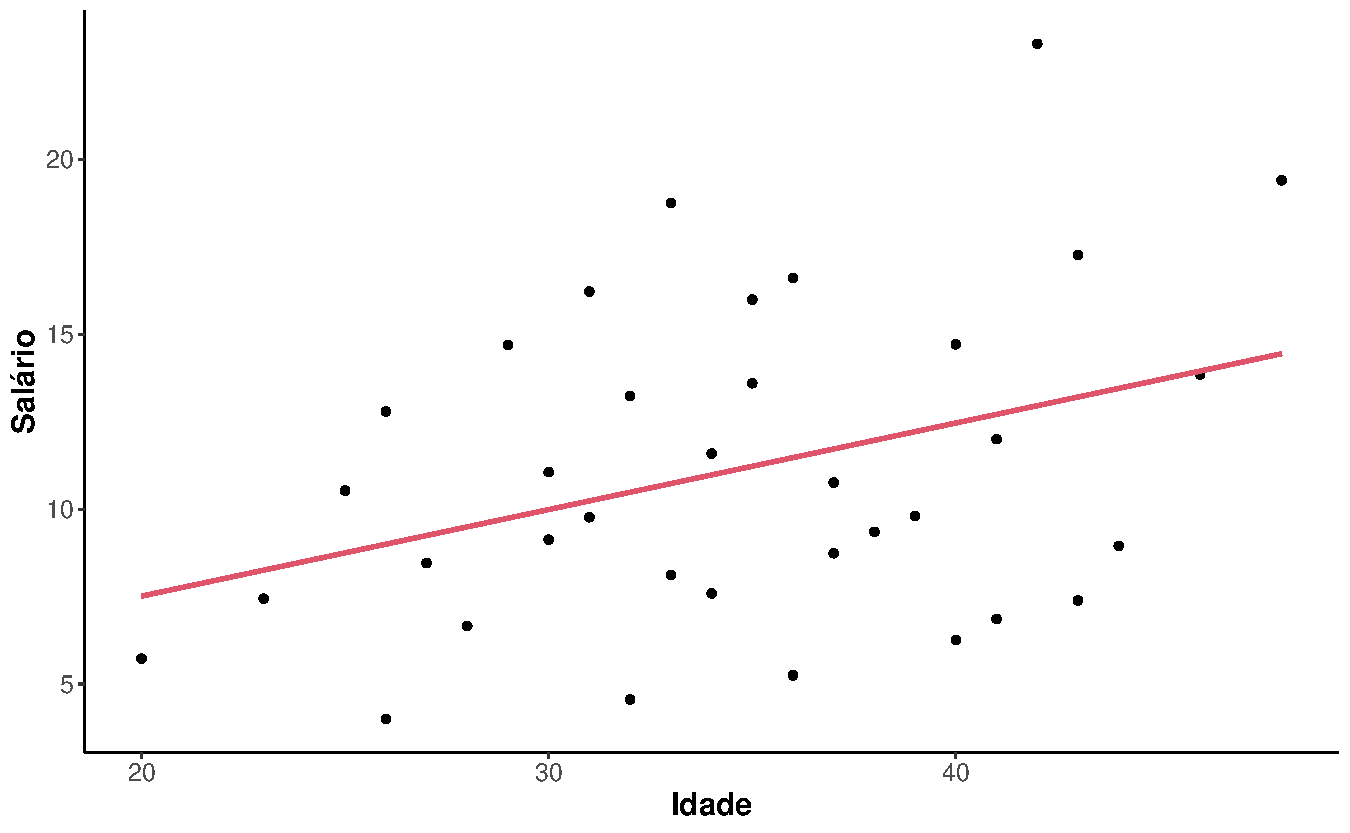
\includegraphics[width=11cm]{encontro2_files/figure-beamer/unnamed-chunk-32-1} 

}

\caption{Diagrama de dispersão para o salário em função da idade.}\label{fig:unnamed-chunk-32}
\end{figure}
\end{frame}

\begin{frame}{Interpretação gráfica}
\phantomsection\label{interpretauxe7uxe3o-gruxe1fica}
\begin{figure}

{\centering 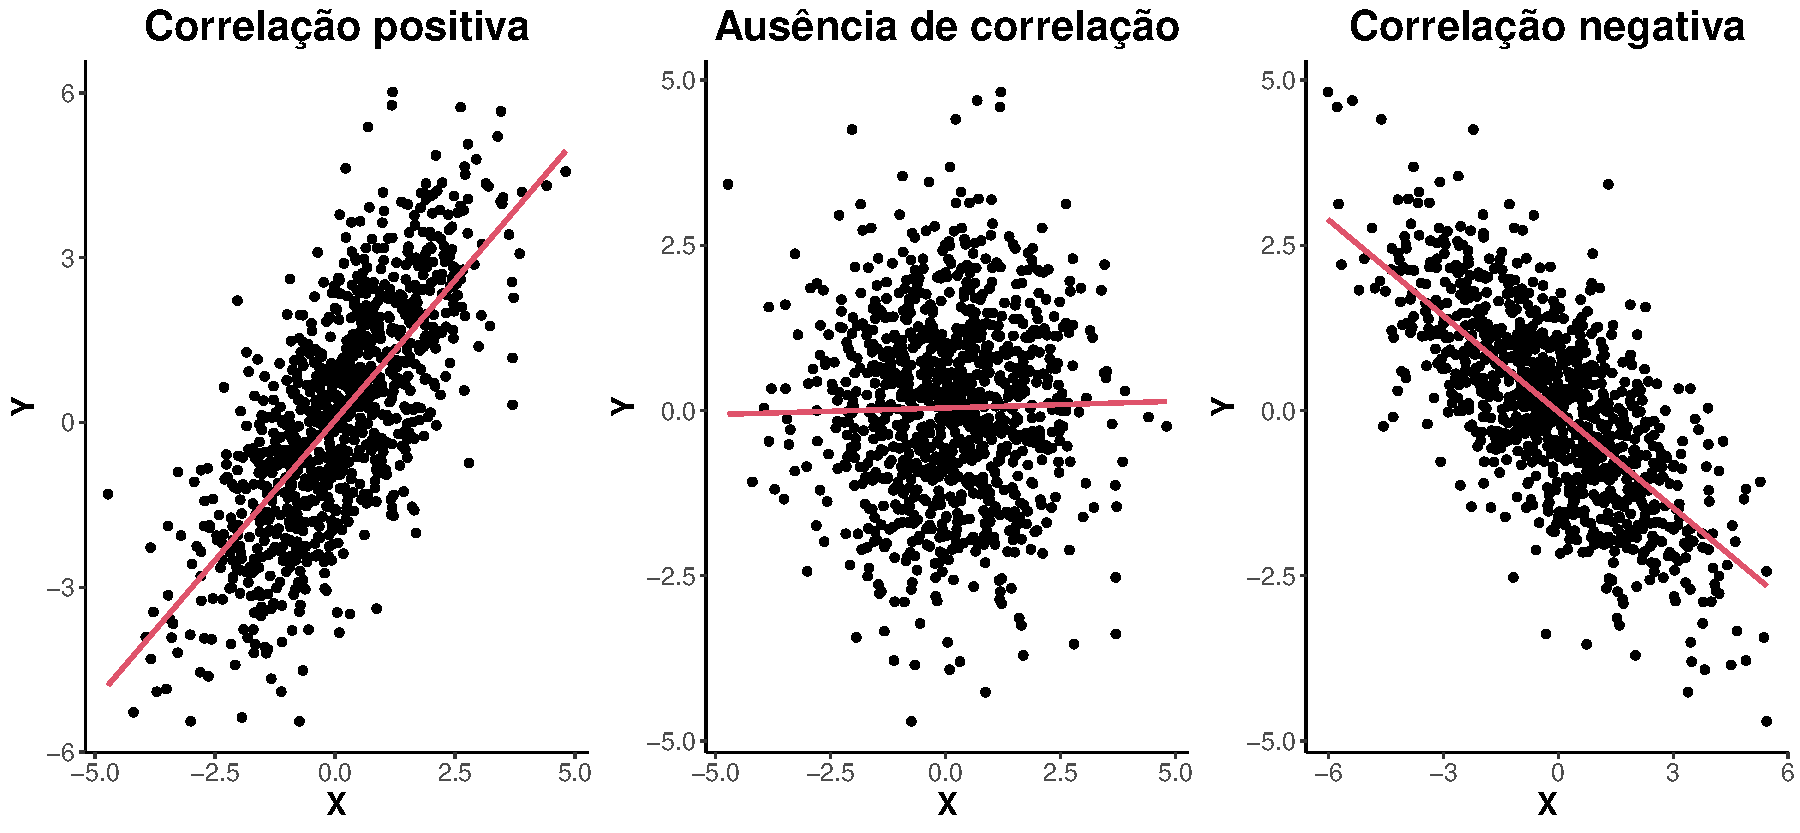
\includegraphics[width=11cm]{encontro2_files/figure-beamer/unnamed-chunk-33-1} 

}

\caption{Avaliação de correlação usando diagramas de dispersão.}\label{fig:unnamed-chunk-33}
\end{figure}
\end{frame}

\begin{frame}{Covariância, correlação e diagrama de dispersão}
\phantomsection\label{covariuxe2ncia-correlauxe7uxe3o-e-diagrama-de-dispersuxe3o}
\textbf{Exemplo}

\begin{itemize}
\tightlist
\item
  Considere as variáveis peso (\(Y_1\)) e altura (\(Y_2\)) de um
  conjunto de 10 indivíduos.
\end{itemize}

\[Y_1: 60,09; 57,97; 54,12; 70,76; 59,74; 50,41; 58,19; 65,35; 71,18; 54,76\]

\[Y_2: 1,54; 1,62; 1,52; 1,76; 1,63; 1,52; 1,65; 1,67; 1,66; 1,57\]

\begin{itemize}
\item
  \(\overline{Y_1} = 60,26\); \(\overline{Y_2} = 1,61\).
\item
  \(Var(Y_1) = 47,8\); \(Var(Y_2) = 0,006\).
\item
  Obtenha a covariância, coeficiente de correlação e o diagrama de
  dispersão.
\end{itemize}
\end{frame}

\begin{frame}{Covariância, correlação e diagrama de dispersão}
\phantomsection\label{covariuxe2ncia-correlauxe7uxe3o-e-diagrama-de-dispersuxe3o-1}
\textbf{Exemplo}

\[
\textrm{Cov}(y_1, y_2) = \frac{1}{10 - 1} \displaystyle \left \{ \left [ (60,09 - 60,26)\cdot (1,54 - 1,61) \right ] + ... + \left [ (57,76 - 60,26)\cdot (1,57 - 1,61)) \right ] \right \}
\]

\[
\textrm{Cov}(y_1, y_2) = 0,44
\]

\[
r  = \frac{0,44}{\sqrt{47,8\cdot 0,006}} = 0,82
\]
\end{frame}

\begin{frame}{Covariância, correlação e diagrama de dispersão}
\phantomsection\label{covariuxe2ncia-correlauxe7uxe3o-e-diagrama-de-dispersuxe3o-2}
\textbf{Exemplo - digrama de dispersão}

\begin{figure}

{\centering 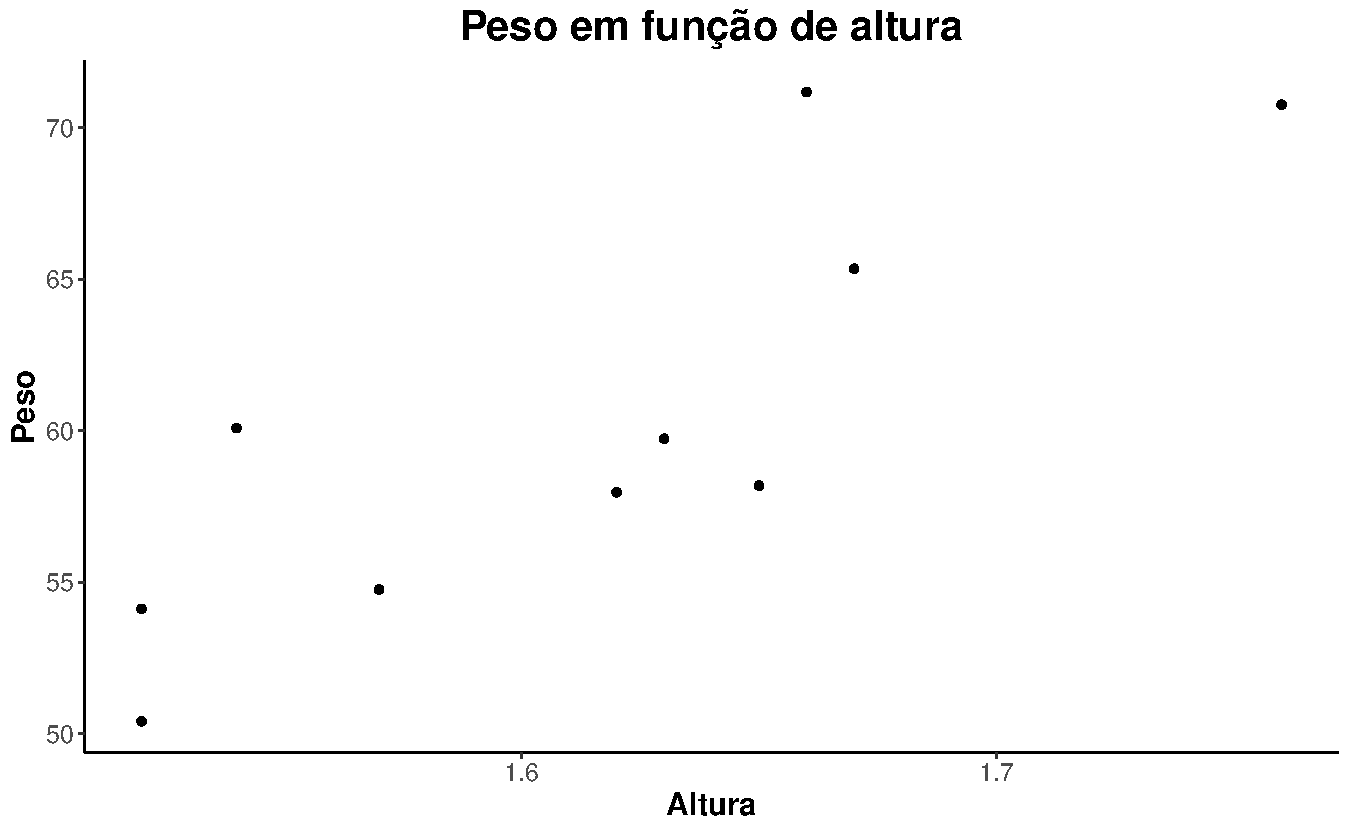
\includegraphics[width=0.65\linewidth]{encontro2_files/figure-beamer/unnamed-chunk-34-1} 

}

\caption{Diagrama de dispersão para peso e altura.}\label{fig:unnamed-chunk-34}
\end{figure}
\end{frame}

\begin{frame}{Covariância, correlação e diagrama de dispersão}
\phantomsection\label{covariuxe2ncia-correlauxe7uxe3o-e-diagrama-de-dispersuxe3o-3}
\textbf{Exemplo - digrama de dispersão}

\begin{figure}

{\centering 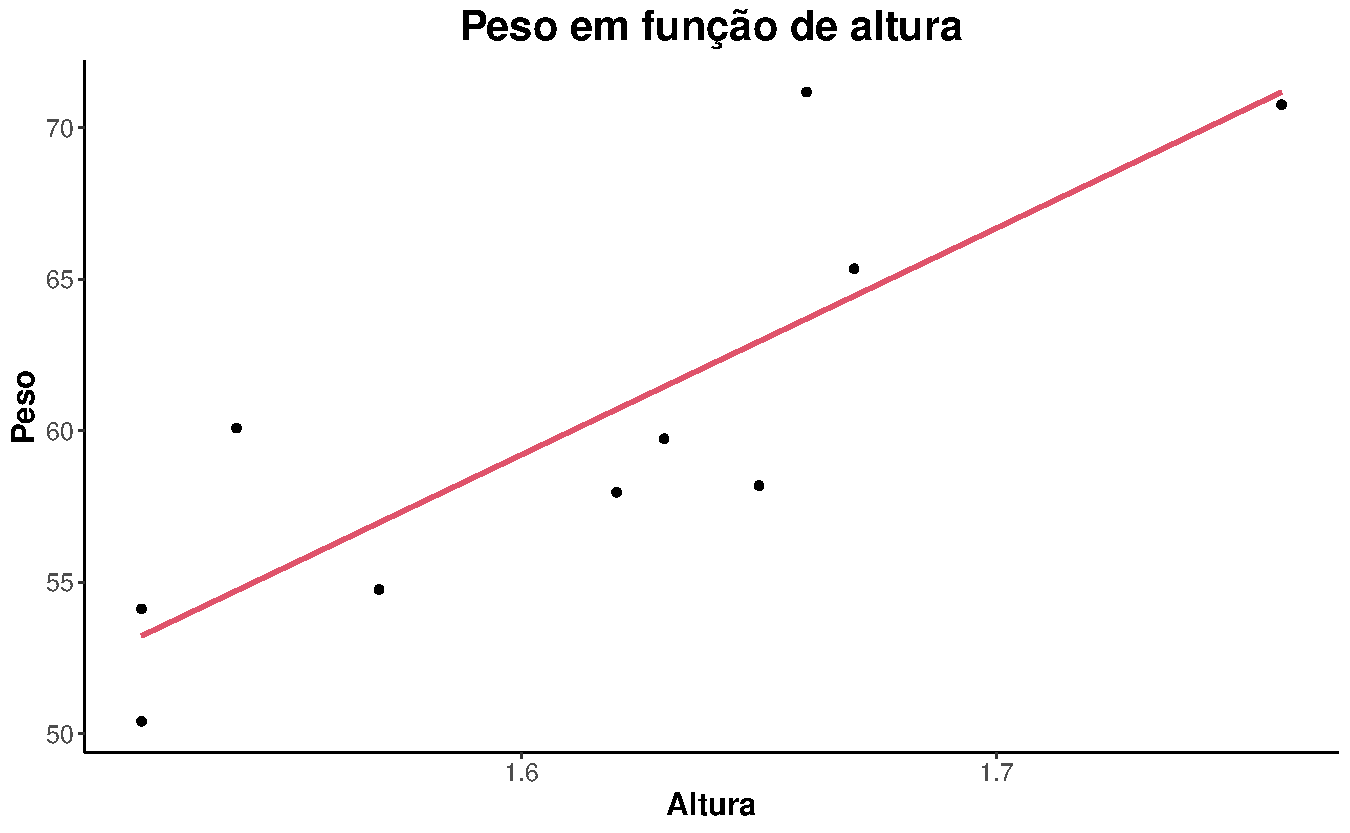
\includegraphics[width=0.65\linewidth]{encontro2_files/figure-beamer/unnamed-chunk-35-1} 

}

\caption{Diagrama de dispersão para peso e altura com linha de tendência linear.}\label{fig:unnamed-chunk-35}
\end{figure}
\end{frame}

\section{Análise bivariada para uma variável qualitativa e uma
quantitativa}\label{anuxe1lise-bivariada-para-uma-variuxe1vel-qualitativa-e-uma-quantitativa}

\begin{frame}{Análise bivariada para uma variável qualitativa e uma
quantitativa}
\phantomsection\label{anuxe1lise-bivariada-para-uma-variuxe1vel-qualitativa-e-uma-quantitativa-1}
\begin{itemize}
\item
  Neste caso estamos interessados em avaliar se os valores da variável
  numérica estão associados com os níveis da variável categórica.
\item
  Podemos usar \textbf{medidas descritivas} para os valores dentro de
  cada um dos níveis da variável categórica.
\item
  Para representar graficamente esta situação podemos criar um
  \textbf{box-plot} da variável numérica para cada nível do fator de
  interesse.
\end{itemize}
\end{frame}

\begin{frame}{Tabela de medidas descritivas para níveis de um fator}
\phantomsection\label{tabela-de-medidas-descritivas-para-nuxedveis-de-um-fator}
\begin{longtable}[]{@{}cccc@{}}
\caption{Medidas descritivas do salário em função da
região.}\tabularnewline
\toprule\noalign{}
Região & Média & Mediana & Desvio padrão \\
\midrule\noalign{}
\endfirsthead
\toprule\noalign{}
Região & Média & Mediana & Desvio padrão \\
\midrule\noalign{}
\endhead
capital & 11.46 & 9.77 & 5.48 \\
interior & 11.55 & 10.64 & 5.30 \\
outro & 10.45 & 9.80 & 3.15 \\
\bottomrule\noalign{}
\end{longtable}
\end{frame}

\begin{frame}{Box-plot para níveis de um fator}
\phantomsection\label{box-plot-para-nuxedveis-de-um-fator}
\begin{figure}

{\centering 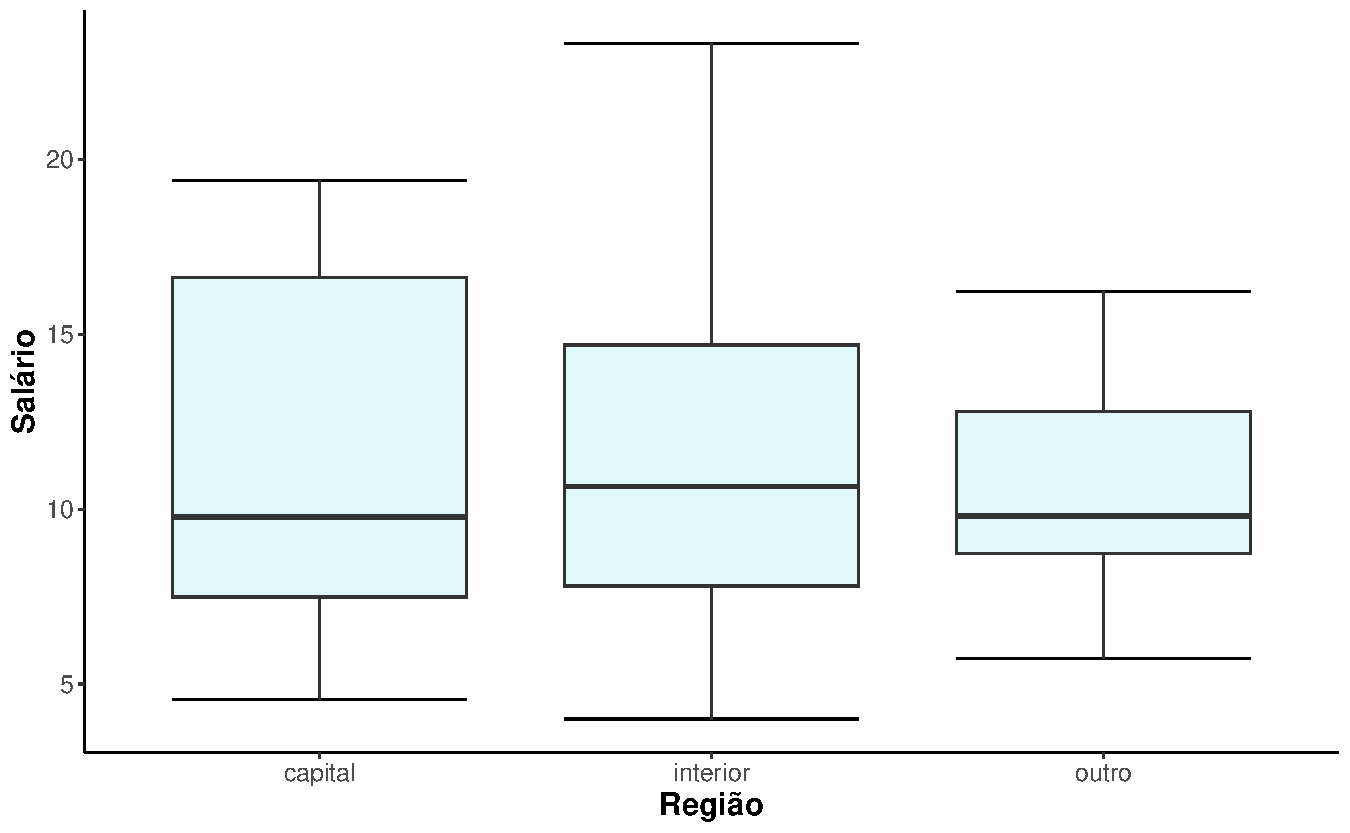
\includegraphics[width=11cm]{encontro2_files/figure-beamer/unnamed-chunk-37-1} 

}

\caption{box-plots para o salário em função da região.}\label{fig:unnamed-chunk-37}
\end{figure}
\end{frame}

\section{Outros tipos de gráficos e
análises}\label{outros-tipos-de-gruxe1ficos-e-anuxe1lises}

\begin{frame}{Outros tipos de gráficos e análises}
\phantomsection\label{outros-tipos-de-gruxe1ficos-e-anuxe1lises-1}
\beginAHalfColumn

\begin{itemize}
\tightlist
\item
  Vimos as alternativas usuais para representação e análise de variáveis
  quantitativas e qualitativas.
\end{itemize}

\vspace{0.3cm}

\begin{itemize}
\tightlist
\item
  Contudo existem diversas situações particulares que exigem análises
  específicas.
\end{itemize}

\endColumns
\beginAHalfColumn

\begin{itemize}
\tightlist
\item
  Algumas casos são: mapas, séries temporais, gráficos de perfil, nuvens
  de palavras.
\end{itemize}

\vspace{0.3cm}

\begin{itemize}
\tightlist
\item
  Também é possível trabalhar com gráficos que representam mais de duas
  variáveis ao mesmo tempo.
\end{itemize}

\vspace{0.3cm}

\begin{itemize}
\tightlist
\item
  Outra possibilidade é combinar gráficos.
\end{itemize}

\endColumns
\end{frame}

\begin{frame}{}
\phantomsection\label{section}
\beginAHalfColumn

\textbf{O que foi visto:}

\begin{itemize}
\tightlist
\item
  Resumos numéricos.
\item
  Medidas de posição central.
\item
  Medidas de posição relativa.
\item
  Medidas de dispersão.
\item
  Análises bivariadas.

  \begin{itemize}
  \tightlist
  \item
    Qualitativa x qualitativa.
  \item
    Quantitativa x quantitativa.
  \item
    Quantitativa x qualitativa.
  \end{itemize}
\end{itemize}

\endColumns
\beginAHalfColumn

\textbf{Próximos assuntos:}

\begin{itemize}
\tightlist
\item
  Revisando conceitos e extraindo informações de um conjunto de dados
  real com R.
\item
  Considerações finais.
\end{itemize}

\endColumns
\end{frame}

\end{document}
